% Style for a MSc paper at Warsaw School of Economics
% Michał Ramsza
% Friday, December 14, 2012

% --- document class and other global stuff ---------------------------
\documentclass[polish, twoside, 12pt, a4paper]{article}

% --- packages --------------------------------------------------------
\usepackage{textcomp}
\usepackage{times}
\usepackage{amsmath}
\usepackage{amsfonts}
\usepackage{amssymb}
\usepackage{amsthm}
\usepackage[T1]{fontenc}
\usepackage[utf8]{inputenc}
\usepackage{graphicx}
\usepackage{xcolor}
\usepackage{enumitem}
\usepackage[polish]{babel}
\usepackage[centering, left=3.5cm, right=2.5cm, textheight=24cm]{geometry}
\usepackage{tikz}
\usepackage{pgf-umlcd}

% --- tikz-----------------------------------------------------------------

\usetikzlibrary{shapes.callouts}

\tikzset{
  level/.style   = { ultra thick, blue },
  connect/.style = { dashed, gray },
  connect_k/.style = { dashed, red },
  notice/.style  = { draw, rectangle callout, callout relative pointer={#1} },
  label/.style   = { text width=2cm }
}


% --- packages for citations ------------------------------------------
\usepackage{natbib}
\AtBeginDocument{\renewcommand{\harvardand}{i}}

% --- package for automatic insertion of R code -----------------------
\usepackage{listings}
\lstset{language=R,%
   numbers=left,%
   tabsize=3,%
   numberstyle=\footnotesize,%
   basicstyle=\ttfamily \footnotesize \color{black},%
   escapeinside={(*@}{@*)}}

% --- support for links -----------------------------------------------	
\usepackage{url}
\usepackage{hyperref}
\hypersetup{colorlinks=true,
            linkcolor=black,
            citecolor=darkgray,
            urlcolor=darkgray,
            pagecolor=darkgray}

% --- support for large tables and other stuff ------------------------	
\usepackage{longtable}
%\usepackage{subfigure} % this package will now work with subcaption package
\usepackage{float}
\usepackage{caption}
\usepackage{subcaption}


% --- definitions for environments -------------------------------------
\theoremstyle{definition}
    \newtheorem{condition}{Assumption}
    \newtheorem{example}{Example}      

\theoremstyle{plain}
    \newtheorem{definition}{Definition}    
    \newtheorem{proposition}{Proposition}
    \newtheorem{theorem}{Theorem}
    \newtheorem{cor}{Corollary}

\theoremstyle{remark}
    \newtheorem{remark}{Remark}

% --- other settings --------------------------------------------------
\linespread{1.5}
\frenchspacing
\sloppy
\allowdisplaybreaks[4]
\raggedbottom
\clubpenalty=10000
\widowpenalty=10000

% --- only if required ------------------------------------------------
\AtBeginDocument{\renewcommand*{\figurename}{Wykres}}
\AtBeginDocument{\renewcommand*{\tablename}{Tabela}}

% ---------------------------------------------------------------------
\begin{document}

% --- strona tytulowa -------------------------------------------------
\begin{titlepage}
\centering


\includegraphics[width=0.66\textwidth]{logo.JPG}

\vspace*{0.5cm}
Studium magisterskie\\
\begin{flushleft}
Kierunek: Finanse i Rachunkowość\\
Specjalność: Finanse przedsiębiorstw\\
Forma studiów: stacjonarne
\end{flushleft}

\vspace*{.5cm}
\rule{0cm}{1cm}\hfill
\begin{minipage}{9cm}
Imie i nazwisko: Hubert Guzera\\
Nr albumu: 61816
\end{minipage}

\vspace*{1cm}
\begin{minipage}{12cm}
\centering
\Large
\textbf{Wykorzystanie modelowania predyktywnego do stworzenia heurystyki optymalizacji decyzji w przedsiębiorstwie}
\end{minipage}

\vspace*{2cm}
\rule{0cm}{1cm}\hfill
\begin{minipage}{9cm}
Praca magisterska napisana\\
w Kolegium Analiz Ekonomicznych\\
w Katedrze Matematyki i Ekonomii Matematycznej\\
pod kierunkiem naukowym\\
dr hab. Michała Ramszy
\end{minipage}

\vfill
Warszawa 2015
\end{titlepage}

\rule{1ex}{0ex}\clearpage


% --- table of contents -----------------------------------------------
\cleardoublepage
\tableofcontents

% --- chapter ---------------------------------------------------------
\cleardoublepage
\section{Wprowadzenie}

Wal-Mart, amerykański gigant handlowy, co godzinę umieszcza w swoich bazach danych 2.5 petabajtów danych, pochodzących z blisko miliona transakcji (\cite{Economist2010}). I nie jest wyjątkiem --- przeciętna ilość danych przechowywanych przez przedsiębiorstwa w Stanach Zjednoczonych jest większa niż zbiory Biblioteki Kongresu (szacowane na 235 terabajtów (\cite{McKinsey2011}). W erze informacji większość z naszych działań trafia na serwery tej bądź innej firmy, w formie historii transakcji, koordynatu GPS czy zdjęcia. 

Często informacje zbierane są przypadkiem --- ze względu na prowadzenie rachunkowości, specyfikę świadczonych usług, lub też względy archiwizacyjne. Jednak wydobycie z nich \textit{wiedzy} może stanowić źródło znaczącej przewagi konkurencyjnej.  Jak wskazują \cite{Brynjolfsson2011}, przedsiębiorstwa podejmujące decyzje na podstawie analizy dużych zbiorów danych (\textit{ang. data driven decision making}) osiągają efektywność o 5-6 proc. większą niż grupa porównawcza. Mają także większy zwrot z kapitału i wycenę rynkową --- krótko mówiąc, radzą sobie lepiej. Nic więc dziwnego, że coraz częściej metody analizy danych (\textit{ang. data analytics}) stają się priorytetem wśród dużych spółek. Skalę popularności analityki biznesowej (\textit{ang. business intelligence}) unaocznia badanie \cite{PwC2014}, według którego 44 proc. prezesów zarządu planuje oparcie rozwoju firmy o inwestycje w tej dziedzinie. 

Ale dzisiejsze zastosowania \textit{big data} to tylko preludium do tego, co czeka nas w przyszłości. Trwający równolegle trend robotyzacyjny spowoduje, że w ciągu 20 lat w przedsiębiorstwie zamiast kierowców będziemy zarządzać flotą autonomicznych pojazdów, a magazynierów zastąpią roboty. Fakt, że Google i Daimler już testują takie auta nie pozwala na nazwanie takiego scenariusza \textit{science-fiction}. Dlatego jak wskazuje \cite{frey2013}, blisko 47 proc. miejsc pracy jest zagrożonych komputeryzacją. Większość z nich to zawody wykonujące rutynowe, mechaniczne czynności, ale postęp technologiczny powoduje, że na tej liście znajdują się też prace wymagające umiejętności kognitywnych i wnioskowania --- jak pracownicy biurowi, analitycy czy operatorzy. 

Mając do czynienia z jednej strony z flotą autonomicznych pojazdów, z a drugiej z petabajtami informacji o tym gdzie i co kupują nasi klienci, możemy znaleźć się w sytuacji, gdzie koordynacja łańcucha dostaw będzie wykraczać poza możliwości człowieka. Dla komputera, obliczenie popytu na podstawie danych i zaplanowanie dostaw będzie relatywnie mniejszym problemem. Potwierdza to The McKinsey Global Institute \cite{McKinsey2011}, który wskazuje, że coraz częściej maszyny będą zastępować ludzi w podejmowaniu decyzji i brać udział w sterowaniu przedsiębiorstwem. W teorii, ze względu na możliwość przeprowadzania złożonych obliczeń i analizy gigabajtów danych, decyzje te będą trafniejsze i poprawią efektywność przedsiębiorstwa. 

Niniejsza praca ma na celu analizę tej hipotezy w sztucznym modelu wieloagentowym. Po pierwsze, poprzez zaproponowanie jednego z wielu możliwych algorytmów optymalizacji działania przedsiębiorstwa poprzez wykorzystanie istniejących technik modelowania predykcyjnego (\textit{ang. predictive analytics}). Po drugie przez sprawdzenie, jak tak podejmowane decyzje będą wpływać na funkcjonowanie przedsiębiorstwa i czy będzie ono funkcjonować efektywniej, niż gdyby zastosować w nim dotychczasowe praktyki biznesowe.


% --- chapter ---------------------------------------------------------
\clearpage

\section{Cel, założenia i podstawy teoretyczne pracy}

Praca ma na celu zaproponowanie heurystyki optymalizacji podejmowania decyzji w przedsiębiorstwie na podstawie modelowania predyktywnego oraz sprawdzenie w modelu wieloagentowym, jak zaimplementowanie takiego algorytmu wpływa na wyniki firmy .  

\subsection{Koncepcja pracy}

Rozważane w pracy przedsiębiorstwo należy do sektora szybko zbywalnych towarów konsumpcyjnych (\textit{ang. fast moving consumer goods, FMCG)} i zajmuje się zarówno ich produkcją, jak i dystrybucją do sklepów detalicznych. Na podstawie historycznych danych o transakcjach i klientach prognozowany będzie krótkoterminowy wolumen sprzedaży w każdym z prowadzonych sklepów. Otrzymana wiedza zostanie wykorzystana do optymalizacji procesów logistycznych, przez co rozumiane jest wybranie tras dostaw i alokację wśród nich wolumenów produktów tak, aby zysk firmy był jak największy. 

W celu zaprezentowania wyniku działania powstałego w ten sposób algorytmu, zostanie zbudowany model wieloagentowy symulujący rynek i zachowania klientów. Z jego pomocą sprawdzimy wpływ działania algorytmu na decyzje firmy oraz jej wyniki finansowe i operacyjne.

\subsection{Podstawy teoretyczne} \label{chapter:teoria}
\subsubsection{Przedsiębiorstwo jako system wieloelementowy} 
Na możliwość wykorzystania modeli wieloagentowych do badania i zarządzania systemami logistycznymi wskazują m.in. \cite{Moyaux2006} czy \cite{Kawa2010}. W swoich pracach zauważyli oni, że  \textit{producenci},  \textit{dostawcy},  \textit{odbiorcy} orazi inni uczestnicy łańcucha logistycznego mogą być opisani jako sieć autonomicznych, współpracujących ze sobą agentów, jak pokazane zostało to na wykresie \ref{fig:siecKawa}. Takie podejście, i wynikająca z niego możliwość wykorzystania modeli wieloagentowych pomaga w rozwiązaniu problemów operacyjnych, na jakie wskazuje \cite{Kawa2010}. Należy bowiem zwrócić uwagę, że w zakresie wyboru tras i zarządzania flotą wieloetapowe łańcuchy dostaw wielu produktów są problemami NP-trudnymi, szczególnie, że decyzje podejmowane lokalnie są współzależne.\footnote{Decyzje podjęte na krańcowych etapach łańcucha wpływają na wcześniejsze lub późniejsze etapy, co \cite{Moyaux2006} opisuje jako m.in. "bullwhip effect".} Ponadto, jak zauważa \cite{Kawa2010}, w sieci przedsiębiorstw pomiędzy dostawcami kolejnych rzędów (tj. fabryki, magazyny, sklepy) może istnieć wiele połączeń które są wobec siebie konkurencyjne. Przykładowo, magazyn może zaopatrywać się w wielu fabrykach. Zastosowanie w tej dziedzinie modeli wieloagentowych pozwala więc na zbadanie, jak decyzje podejmowane na jednym z etapów łańcucha dostaw wpłyną na cały system i innych uczestników.  


% --- figure --------------------------------------------------------
\begin{figure}[hbt]
  \centering
  \begin{subfigure}[t]{0.8\textwidth}
    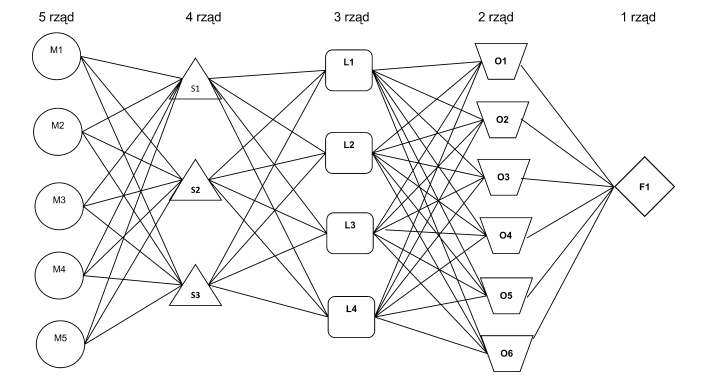
\includegraphics[width=\textwidth]{pictures/siec.png}
  \end{subfigure}
  \captionsetup{margin=10pt,font=small,labelfont=bf,width=.8\textwidth}
  \caption[Łańcuch dostaw w postaci grafu kierunkowego]{Łańcuch dostaw w branży komputerowej przedstawione przez \cite{Kawa2010} jako graf skierowany \textit{Źródło:} \cite{Kawa2010}}\label{fig:siecKawa}.
\end{figure}
% --- figure --------------------------------------------------------

Podejście opiera się na obserwacji, że relacje pomiędzy jednostkami w przedsiębiorstwie są analogiczne do relacji uczestników łańcucha dostaw. \cite{Porter1985} zauważył, że działalność przedsiębiorstwa to de facto sekwencja działań, która na każdym ogniwie zwiększa wartość dla odbiorcy. Zasady funkcjononawia opisywanego przez Portera \textit{łańcucha wartości} są identyczne co do opisywanego przez \cite{Moyaux2006} i \cite{Kawa2010} łańcucha dostaw. Relacje pomiędzy kolejnymi jego elementami można przedstawić w sposób zaproponowany przez \cite{Kawa2010} --- z wykorzystaniem grafu skierowanego, jak zaprezentowano na wykresie \ref{fig:siecKawa}. Podobieństwo to podkreśla fakt, że przedsiębiorstwa poprzez strategię \textit{integracji wertykalnej} swym zasięgiem mogą w rzadkich przypadkach objąć całość łańcucha dostaw.  

Warto zuważyć, że przedsiębiorstwa często dysponują wieloma duplikującymi swoje działania jednostkami \footnote{Dobrym przykładem są tutaj zakłady samochodowe, które mogą produkować dany model w różnych krajach. Zmiana fabryki powoduje przy tym radykalną zmianę łańcucha dostaw.}, przez co łańcuch ten jest nieliniowy i podobne jak w łańcuchu logistycznym problem zarządzania nim będzie problemem NP-trudnym.

Zdefiniowanie jako agentów poszczególnych jednostkek przedsiębiorstwa jest przy tym spójne z określoną przez \cite{Wooldridge1995} charakterystyką agenta, który według ich postulatów posiada : 

	\begin{itemize}
		\item autonomię --- poszczególne jednostki przedsiębiorstwa podążają za strategią i celami narzuconymi przez zarząd, ale mają swobodę w podejmowaniu decyzji operacyjnych.
		\item zdolności do komunikacji --- pomiędzy jednostkami przedsiębiorstwa istnieje asymetria informacji, dlatego komunikują się one zarówno między sobą (raportowanie do zarządu, spotkania) jak i z otoczeniem (relacje z klientami).
		\item reaktywność --- jednostki przedsiębiorstwa reagują na zmiany rynkowe oraz zmiany wewnętrz przedsiębiorstwa, poprzez dostosowywanie decyzji operacyjnych.
	 	\item proaktywność --- jednostki przedsiębiorstwa podejmują inicjatywy mające na celu zwiększyć wartość przedsiębiorstwa, jak działalność innowacyjna bądź ekspansja. 
	\end{itemize}
 
 Dlatego w niniejszej pracy będziemy rozważać model wieloagentowy (zob. rozdział \ref{chapter:model}), w którym według założeń na przedsiebiorstwo składać się będzie wiele powiązanych ze sobą elementów działających w ramach środowiska modelu wieloagentowego. 

\subsubsection{Modelowanie predykcyjne} \label{chapter:statistical} 
W procesach logistycznych i produkcyjnych kluczowym wyzwaniem jest niepewność związana ze zmiennością sprzedaży i jej wartości w chwili $t+1$. Jak wskazuje \cite{James2013} do zmniejszenia niepewności możemy wykorzystać metody statystyczne, poprzez prognozowanie sprzedaży. Jak stwierdza \cite{James2013}, zakładając, że dysponujemy zbiorem $n$ obserwacji $p$ zmiennych, możemy zbadać ich relację ze zmienną wyjaśnianą $y$ i otrzymać \textit{model}, który dla nowych --- nieanalizowanych wcześniej --- obserwacji $x_1,x_2..x_n$  zwraca przewidywaną wartość zmiennej objaśnianej $\hat{y}$. Różnorodne metody modelowania zmiennej objaśnianej (wspólnie nazywane przez \cite{James2013} uczeniem statystycznym, \textit{ang. statistical learning}) mogą być wykorzystane do modelowania predykcyjnego, tj. przewidywania przyszłych wydarzeń na podstawie przeszłej historii danych, w tym również przyszłego wolumenu sprzedaży w przedsiębiorstwie. 

Zastosowanie metod \textit{statistical learning} w przedsiębiorstwach potwierdza \cite{Buckinx2007}, który wskazywał na możliwość prognozowania lojalności klienta na podstawie wewnętrznych danych o transakcjach, oraz \cite{Davenport2011}, który opisuje szereg studiów przypadku firm, w których wykorzystuje się istniejące dane o transakcjach do przewidywania przyszłych zakupów klientów. Jednym z podanych przez niego przykładów jest Tesco, które na podstawie zebranych danych przewiduje, jakich produktów będzie potrzebował w najbliższym czasie \footnote{W aspekcie praktycznym, można zdobyć taką informację obserwując zakupy klientów o podobnym profilu i dostrzegając w zakupach pewne wzorce.}, i odpowiednio wcześnie wysyła mu bony na te produkty. \footnote{Klient widząc atrakcyjną ofertę na produkty których właśnie potrzebuje będzie bardziej skłonny do zrobienia zakupów akurat w Tesco.}. Również podczas panelu \textit{Strategia B2C w erze Big Data --- jak wykorzystać potencjał danych} na XXV Forum Ekonomicznego w Krynicy przedstawicielie polskiego biznesu zwracali uwagę na szerokie wykorzystanie modelowania predykcyjnego również w nasz gospodarce. \footnote{Jednak jak zwracano uwagę, \textit{big data}\ i \textit{modelowanie predykcyjne}\ służą głównie do pozyskiwania danych do późniejszego manualnego przetworzenia i wyciągnięcia z nich wniosków, a nie automatyzacji podejmowania decyzji, co rozważamy w tej pracy}

Podane przykłady dają nam podstawy, żeby w przypadku optymalizowanego przedsiębiorstwa zakładać, że dane o każdej transakcji są zapisywane wraz z niektórymi danymi osobowymi klienta \footnote{To stwierdzenie opiera się na opisywanym przez \cite{Davenport2011} przypadku Tesco i zastosowanej przez nich metody zbierania danych. Możliwość zbierania danych o transakcjach określonego klienta daje karta lojalnościowa (lub konto, w przypadku e-commerce), na którą rejestrowana jest każda transakcja. Praktyką jest, żeby przy okazji tworzenia karty lojalnościowej zbierać informacje o kliencie w ankiecie (zakres danych zależy od praktyki korporacyjnej). Dzięki temu, przedsiębiorstwa są w stanie przypisać do zakupów dane osobwe jak płeć, miejsce zamieszkania, wykształcenie etc.}, a cały zbiór danych może być wykorzystany do przewidywania sprzedaży w chwili $t + 1$. Dlatego w pracy będziemy zakładać, że dla każdej transkacji w sklepie dysponujemy zbiorem informacji, zawierące dane o transakcji (\textit{data, miejsce, rodzaj płatności}), produkcie (\textit{nazwa produktu, cena, ilość}) oraz dane opisujące klienta (\textit{płeć, wiek, zarobki, wykształcenie}).

Podejście zastosowane w pracy zakłada, że na podstawie tak uzyskanego zbioru danych prognozujemy kolejno następujące wartości, które łącznie dadzą nam informacje o sprzedaży w danym sklepie w chwili $t+1$:
	\begin{itemize} 
		\item liczebność poszczególnych grup klientów \footnote{Przez \textit{poszczególne grupy klientów} rozumiemy klientów o wspólnych cechach.} odwiedzających sklep w chwili $t+1$,
		\item[]oraz, w zależności od zastosowanego podejścia,

		\item prawdopodobieństwo z jakim klient o danej charakterystyce kupi produkt,
		\item produkt wybrany przez danego klienta. 
	\end{itemize}

Dwa wymienione podejścia różnią się fundamentalnie jeśli chodzi o to, czym jest zmienna objaśniana. Jak wskazuje \cite{James2013}, zmienna objaśniana może przyjąć różne dziedziny --- m.in. zmiennej binarnej (1/0), prawdopodobieństwa, \textit{log odds} lub klasy --- i z tego względu każdy z przypadków różni się metodami, które możemy zastosować. W pierwszym przypadku chcemy otrzymać liczbę, której przedział powinien być ograniczony w zakresie $(0,1)$. W drugim przypadku, zależy nam nam przyporządkowaniu rekordu do którejś z już określonych klas. Według sugestii \cite{James2013} i \cite{hastie2001}, do prognoz w modelu zastosowane zostaną następujące metody:

	\begin{itemize} 
		\item do prognozowania liczby klientów --- regresję metodą OLS (\textit{metoda najmniejszych kwadratów, ang. ordinary least squares}),
		\item do prognozowania prawdopodobieństwa zakupu --- regresję logistyczną (\textit{ang. logistic regression}),
		\item do prognozowania wyboru produktu --- metody klasyfikacyjne np. K-najbliższych sąsiadów (\textit{ang. K-nearest neighbours}), drzewa klasyfikacyjne (\textit{ang. classification tree}),
	\end{itemize}
	jak również metody nie służące bezpośrednio do modelowania $\hat{y}$, jednak wspierające proces predykcyjny oraz symulowanie decyzji konsumenckich w modelu wieloagentowym:
	\begin{itemize} 
		\item pomiar odległości (\textit{ang. distance scaling}), poprzez liczenie odległości euklidesowej (\textit{ang. euclidean distance}) pomiędzy dwoma zbiorami danych i stworzenie obliczenie macierzy niepodobieństwa (\textit{ang. dissmiliarity matrix}),
		\item eliminację zmiennych (\textit{ang. backward elimination}), która jest jednym z podejść wyboru podzbiorów (\textit{ang. subset selection}) do selekcji zmiennych wyjaśniających, które wspólnie tworzą najlepszy model,
		\item prawdopodobieństwo warunkowe do przewidywania, jakie cechy będą mieli konsumenci odwiedzający sklep w $t+1$.
	\end{itemize}	


\newpage

\subsubsection{Zadanie optymalizacyjne} \label{chapter:zadanie}

Rozważmy przedsiebiorstwo, które za argumentacją przedstawioną w rozdziale \ref{chapter:teoria} oraz obserwacjami  \cite{Moyaux2006} i \cite{Kawa2010} przedstawiamy jako system składający się z wielu elementów. Zakładamy, że rozważane przedsiębiorstwo składa się ze:
	\begin{itemize} 
		\item skończonego zbioru \textit{fabryk} oznaczonych przez FA, z generycznym elementem $fa_n \in FA$,
		\item skończonego zbioru \textit{magazynów} oznaczonych przez MA, z generycznym elementem $ma_n \in MA$,
		\item skończonego zbioru \textit{sklepów} oznaczonych przez SK, z generycznym elementem $sk_n \in SK$,
		\item oraz \textit{zarządu}, pełniący rolę centralnego koordynatora.
	\end{itemize}

Jak zauważył \cite{Kawa2010}, jeśli rozpatrujemy przedsiębiorstwo pod kątem procesów logistycznych, możemy zaobserować, że jednostki przedsiębiorstwa będą wspólnie tworzyć graf skierowany $S = \{FA \cup MA \cup SK, D\}$ (zob. wykres \ref{fig:firma_graf}), gdzie jednostki przedsiębiorstwa $fa \in FA, ma \in MA, sk \in SK$ będą wierzchołkami grafu, a trasy dostaw pomiędzy jednostkami będą krawędziami grafu  $d \in D = D_1 \cup D_2 = \{(i,j) : i \in FA, j \in MA\} \cup \{(i,j) : i \in MA, j \in SK\}$. 

% --- figure --------------------------------------------------------
\begin{figure}[hbt]
  \centering
\begin{center}
\begin{tikzpicture}
   % Draw all levels
  \draw[level] (0,0) -- node[above] {fabryka  $fa_1$} node[below] {($k_{fa_1}$)}  (2,0);
  \draw[connect] (2,0)  -- (3,-1);
  \draw[connect] (2,0) -- (3,1);
  \draw[connect] (2.5,0.75) -- (2.5,0.75) node[below] {$d_1$};
  \draw[connect] (2.5,-0.75) -- (2.5,-0.75) node[below] {$d_2$};
  \draw[level]   (3,1)  -- node[above] {magazyn  $ma_1$} node[below] {($k_{ma_1}$)} (5,1);
  \draw[level]   (3,-1) -- node[above] {magazyn $ma_2$} node[below] {($k_{ma_2}$)} (5,-1);
  \draw[connect] (5,1)    -- (6,2) (5,1) -- (6,0) (5,1) -- (6,-2) (5,1);
  \draw[connect] (5,-1)    -- (6,2) (5,-1) -- (6,0) (5,-1) -- (6,-2) (5,-1);
  \draw[level]   (6,2)  -- node[above] {sklep $sk_1$} node[below] {($k_{sk_1}$)}  (8,2); 
  \draw[level]   (6,-2)  -- node[above] {sklep $sk_2$}node[below] {($k_{sk_1}$)}  (8,-2);
  \draw[level]   (6,0)  -- node[above] {sklep $sk_3$}node[below] {($k_{sk_1}$)}  (8,0);
  \node[text width=5cm] at (11,2.5) {  $ w_1 = {fa_1,ma_1,sk_1, d_1,d_3}  $};
  \node[text width=5cm] at (11,1.5) {  $ w_2 = {fa_1,ma_1,sk_2, d_1,d_4}  $};
  \node[text width=5cm] at (11,0.5) {  $ w_3 = {fa_1,ma_1,sk_3, d_1,d_5}  $};
  \node[text width=5cm] at (11,-0.5) {  $ w_4 = {fa_1,ma_2,sk_1, d_2,d_6}  $};
  \node[text width=5cm] at (11,-1.5) {  $ w_5 = {fa_1,ma_2,sk_2, d_2,d_7}  $};
  \node[text width=5cm] at (11,-2.5) {  $ w_6 = {fa_1,ma_2,sk_3, d_2,d_3}  $};
  % Draw labels
  \node[label] at (1,3.5)  {\textit{Fabryki}};
  \node[label] at (4,3.5)  {\textit{Magazyny}};
  \node[label] at (7.5,3.5)  {\textit{Sklepy}};
  \node[label] at (10.75,3.5)  {\textit{Ścieżki}};
  % Draw annotations
\end{tikzpicture}
\end{center}
  \captionsetup{margin=10pt,font=small,labelfont=bf,width=.8\textwidth}
  \caption[Rozważane przedsiębiorstwo przedstawione jako graf kierunkowy]{Rozważane przedsiębiorstwo przedstawione jako graf kierunkowy. \textit{Źródło:} opracowanie własne.}\label{fig:firma_graf}
\end{figure}
% --- figure --------------------------------------------------------

Planowanie produkcyjno-logistyczne w tak opisanym przedsiębiorstwie będzie polegało na alokacji wolumenów produkcji na poszczególne ścieżki $w \in W = (d_1,d_2)$, gdzie $d_1 = (fa,ma)$, a $d_2=(ma,sk)$. 

Należy zaznaczyć, że optymalizacja alokacji wolumenów dostaw na ścieżkach zamiast na krawędziach ma znaczenie praktyczne dla przedsiębiorstw, szczególnie międzynarodowych. Dzisiejsze trendy globalizacyjne spowodowały, że często produkcja w danym kraju trafia na kilka rynków, a każda z partii musi być dostosowana do warunków rynków lokalnych \footnote{Rozumieny przez to zarówno aspekty regulacyjno-prawne, jak i różnice w preferencjach klientów związane z lokalną kulturą (przykładowo, samochody z bydlęcą skórą nie będą hitem na rynku indyjskim). Dodatkowo, w niektórych branżach, jak samochodowej, można dostosowywać specyfikację zamawianego produktu podczas zakupu. W takim przypadku również należy zapewnić, że trafi on do miejsca docelowego.}. Aby to umożliwić, w momencie produkcji produkt musi mieć określone miejsce docelowej dostawy. W logice grafu oznacza to, że przedsiębiorstwo musi z góry określić ruch produktu na całej ścieżce, a nie tylko na fragmencie ścieżki do następnej krawędzi. Drugie podejście mogłoby spowodować, że kierowanie produktu do miejsca docelowego byłoby utrudnione i dodawałoby kompleksowość operacyjną żeby kontrolować proces. 

\paragraph{Równanie zysku przedsiębiorstwo}\mbox{}\\

W tak zdefiniowanym grafie proces logistyczny odbywa się przepływem wdłuż krawędzi $D$, a z każdym z elementów grafu $ j \in S$ związany jest koszt przepływu $k_j = f_j(x_j)$\footnote{Warto zauważyć, że koszt przesyłu nie oznacza tylko kosztów transportu, ale także kosztów produkcji w fabryce, kosztów magazynowania oraz kosztów obsługi procesów sprzedaży w sklepie. Dlatego koszt $f_j$ będzie definiowany nie tylko na krawędziach $D$, ale każdym elemencie grafu $S$ --- zarówno wierzchołków, jak i krawędzi.}, gdzie $f$ jest dowolną funkcją kosztu, $j$ rozważanym elementem grafu $S$, a $x_j$ wolumenem produkcji przechodzącym przez dany element. 

Sprzedaż towarów przepływających przez graf następuje w sklepach. Zakładając, że przedsiebiorstwo nie stosuje dyskryminacji cenowej, cena produktu będzie globalna i stała \footnote{Rozumiemy przez to, że cena jest identyczna dla wszystkich klientów, dla wszystkich sklepów oraz wszystkich okresów czasu $t$.}. Przychód $r$ w każdym ze sklepów $sk \in SK$ przy cenie $p$ będzie równy $r = p \times q_{sk}$, gdzie $q$ to sprzedaż w wybranym sklepie $sk$ \footnote{Warto zauważyć, że sprzedaż $q_j$ nie jest tym samym co wolumen $n_j$, ponieważ dostarczenie towaru do sklepu nie gwarantuje jego sprzedaży.}. 

Dla całego systemu funkcja zysku systemu $P_s$ zadana równaniem (\ref{eq:zysk}) będzie zależała przede wszystkim od alokacji wolumenów pomiędzy poszczególne elementy grafu,

\begin{equation} \label{eq:zysk}
P_s = \sum\limits_{sk \in SK} p \times q_{sk} - \sum\limits_{j \in S} f_j(x_j),
\end{equation}
 gdzie $p$ to stała cena, $q_{sk}$  sprzedaż w sklepie $sk \in SK$ spełniająca warunek $q_{sk} \le x_{sk}$ \footnote{Sprzedaż w sklepie nie może być większa niż wolumen dostaw który trafił do sklepu.}, a $f_j$ to dowolna funkcja kosztu zależna od wolumenu $x_j$ w elemencie grafu $j \in S$.

Zadanie maksymalizacji byłoby względnie proste \footnote{Pomijając aspekt złożoności obliczeniowej.}, gdybyśmy mieli doskonałą informację na temat poziomu sprzedaży w każdym ze sklepów w chwili $ t + 1 $. Na taką wiedzę nie możemy liczyć ani w tej pracy, ani w w rzeczywistości, dlatego rozwiązaniem proponowanym w niniejszej pracy jest zastosowanie modelowania predykcyjnego (\textit{predictive analytics}), w celu prognozowania liczby klientów i ich wyborów w każdym ze sklepów w najbliższych okresach czasu. \footnote{Obecnie w przedsiębiorstwach rzadko stosuje się zaawansowane sposoby prognozowania sprzedaży (\textit{predictive analytics}), a zarządzanie dostawami odbywa się raczej metodą manualnego uzupełniania zapasów.} 

Ponadto, jak warto zauważyć, nie możemy liczyć na to, że funkcja kosztu $f_j$ będzie liniowa. Empiryczna obserwacja powszechności efektów skali w każdym z sektorów gospodarki każe nam zakładać, że funkcja kosztu będzie dowolną funkcją nieliniową. Warto przy tym zauważyć, że efekty skali mogą być zarówno dodatnie, jak i ujemne, jak również mogą występować wspólnie \footnote{Dodatnie gdy produkcja będzie mniejsza niż optymalny poziom produkcji, a ujemne po przekroczeniu optymalnych mocy produkcyjnych.}.

Trzecim aspektem, który trzeba wziąć pod uwagę jest złożoność obliczeniowa. Nawet dla prostego układu, lecz wolumenu produkcji ponad 1000 sztuk sprawdzenie zysku w przypadku wszystkich kombinacji alokacji wymaga olbrzymiej liczba iteracji --- liczba kombinacji będzie liczbą Strilinga II rodzaju. Mimo znaczącego wzrostu mocy komputerów w ostatnich latach, wolumeny produkcji w dużych przedsiębiorstwach oraz złożoność tras logistycznych sprawia, że to podejście jest kompletnie niepraktyczne i należy szukać alternatywnych podejść, upraszczających problem.

\subsection{Proponowany algorytm optymalizacyjny} \label{chapter:algorytm}

W proponowanym algorytmie optymalizacyjnym wykorzystujemy fakt, że dzięki modelowaniu predyktywnemu możemy prognozować wolumen sprzedaży $q_{sk}$ w każdym ze sklepów $sk \in SK$. Ponieważ równolegle zakładamy brak stosowania dyskryminacji cenowej, część przychodowa równania (\ref{eq:zysk}) będzie nam znana. Możemy ją oznaczyć jako stałą $r_s$, oznaczającą  przychód całego systemu.  

\begin{equation} \label{eq:przychodsystemu}
P_s = r_s - \sum\limits_{j} f_j(x_j).
\end{equation}

Ponieważ w rozdziale \ref{chapter:zadanie} stwierdziliśmy, że ze względów biznesowych naszym celem jest optymalizacja alokacji wolumenu na ścieżkach, zauważmy, że $x_j$ będzie równe $\sum\limits_{w:j \in w} x_w$, sumie wolumenów $x_w$ na wszystkich ścieżkach $w \in W$ przechodzących przez element grafu $j \in S$, co oznaczamy z niewielkim nadużyciem zapisu jako $j \in w$, dzięki czemu równanie \label{eq:przychodsystemu} możemy zapisać jako: 

\begin{equation} \label{eq:przychodsystemu}
P_s = r_s - \sum\limits_{j} f_j(\sum\limits_{w:j \in w} x_w).
\end{equation}

Dzięki temu przekształceniu możemy wyznaczyć gradient funkcji zysku

\begin{equation} \label{eq:gradient}
\bigtriangledown P_s  = [\frac{\partial P_s}{\partial x_{w_1}}...\frac{\partial P_s}{\partial x_{w_n}}]
\end{equation}
gdzie $n$ to liczba ścieżek w zbiorze $W$.

Zauważmy, że jeśli obliczymy gradient w punkcie, wskaże on nam kierunek najszybszych wzrostów wartości funkcji zysku $P_s$ w zależności od ulokowania kolejnej jednostki produktu na wybraną ścieżkę. Proponowany algorytm wykorzystuje tę właściwość i zakładajac, że działanie algorytmu zaczyna się, gdy każda ze ścieżek $w \in W$ jest pusta, tj. każde $x_{w}=0$, jego działanie składa się z podanych niżej kroków. Dla przejrzystości zapisu przez $\chi_w$ będziemy oznaczali wektor $(x_{w_1},\ldots,x_{w_n})$. 

\clearpage

\begin{enumerate} 
	\item[] Ustal punkt startowy $\chi = (0,\ldots,0)$.
	\item Wyznacz funkcję zysku $P_s$ (symbolicznie).
	\item Wyznacz gradient $\bigtriangledown P_s$ (symbolicznie).
	\item[] Początek pętli
	\item Oblicz gradient w punkcie $\chi$. 
	\item Dla każdego elementu  $\bigtriangledown P_s$ sprawdź
		\begin{itemize}
			\item czy odpowiadająca mu wartość pochodnej cząstkowej jest mniejsza od $0$ (optymalizacja),
			\item czy dodanie kolejnego produktu do ścieżki spowoduje, że w sklepie leżącym na ścieżce przestanie być spełniany warunek $q_{sk} \le x_{sk}$ \footnote{Wolumen dostaw będzie większy niż prognozowany wolumen sprzedaży.} (ograniczenia). 
		\end{itemize}
	\item Jeśli którykolwiek z powyższych jest prawdą, "usuń" \footnote{Usunięcie oznacza, że na tej współrzędnej nie będziemy już dodawać towaru w kolejnych iteracjach.} ścieżkę z wektora  $\bigtriangledown P_s(\chi)$. 
	\item Jeśli wektor $ \bigtriangledown P_s(\chi)$ nie jest pusty, z pozostałych elementów, wybierz ścieżkę o największej wartości poprzez dodanie $1$ na współrzędnej i zmień wektor $\chi$.
	\item Powtórz od kroku 3. dopóki wektor $\bigtriangledown P_s(\chi)$ nie będzie pusty.
\end{enumerate}

Działanie algorytmu w standarcie UML zaprezentowane zostało na wykresie \ref{fig:diagramoptymalizacyny}.

\begin{figure}
  \centering
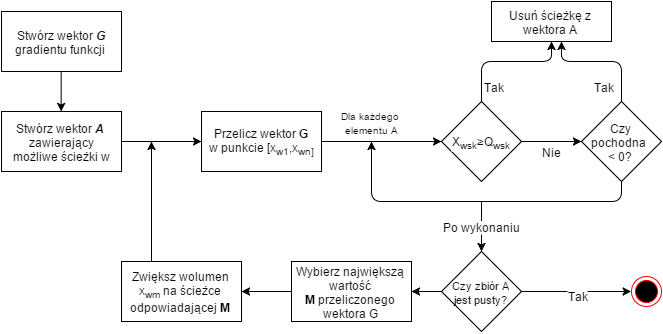
\includegraphics[width=\linewidth]{pictures/diagramoptymalizacyny.png}
  \caption{Proponowany algorytm optymalizacyjny}
  \label{fig:diagramoptymalizacyny}

\end{figure}

\subsection{Cechy algorytmu optymalizacyjnego} \label{chapter:cechy}

Algorytm działający według reguł opisanych w rozdziale \ref{chapter:algorytm} będzie heurystyką, ponieważ kierując się najszybszymi wzrostami w punkcie obliczania gradientu może ominąć maksimum globalne, przez co nie gwarantuje znalezienia najlepszej alokacji w przypadku wystąpienia nietypowych funkcji kosztu. Gwarantuje za to znalezienie aproksymacji maksimum lokalnego i zakończenie pętli \footnote{Tj. nie ma możliwości, żeby iterował w nieskończoność.}. Biorąc pod uwagę, że w aspekcie praktycznym większość funkcji kosztów nie będzie miało nietypowych kształtów, algorytm też powinien być w zupełności wystarczający do większości zastosowań optymalizacyjnych w praktyce.

Ograniczeniem algorytmu jest to, że szukając kolejnych optymalnych punktów operuje on wyłącznie na dyskretnych wartościach $x_w$ (zamiast ciągłych). Wynika to z założenia, że w procesach logistycznych nie możemy przekroić i przetransportować pół produktu, a nawet ładunek drobnicowy będzie miał swoją jednostkę najmniejszego możliwego transportu, jak paleta, tona, kontener etc. 

Algorytm nie oblicza wszystkich możliwych kombinacji alokacji wolumenów, a używa gradientu do oszacowania najbardziej opłacalnej trasy dla każdego z produktów, dlatego czas jego wykonania będzie znacznie krótszy w stosunku do algorytmu obliczającego wszystkie możliwe sytuacje. Liczba iteracji potrzebnych do kalkulacja zysku w przypadku każdej możliwej kombinacji alokacji będzie liczbą Stirlinga II rodzaju, a w przypadku algorytmu maksymalna liczba iteracji będzie iloczynem liczby produktów oraz liczby ścieżek. \footnote{W praktyce będzie mniejsza, ponieważ algorytm pozbywa się nierentownych i zapełnionych ścieżek.}. 

Warto zwrócić uwagę na ciekawą właściwość algorytmu. Gdy przez skalę działalności firmy jej graf będzie bardzo rozbudowany, sposób działania algorytmu pozwala rozważać tylko najbardziej prawdopodobne trasy, zamiast wszystkich. Pozwoli to zmniejszyć liczbę iteracji, jednocześnie zachowując integralność grafu. Inne metody, które w większym stopniu opierają się na iteracjach po elementach grafu, do osiągnięcia analogicznego efektu wymagałyby zmiany struktury grafu, co jest rozwiązaniem niepraktycznym i może w wielu przypadkach zaburzyć wynik. 



% --- chapter ---------------------------------------------------------
\clearpage

\section{Model} \label{chapter:model}

W celu sprawdzenia działania algorytmu zbudowany został model wieloagentowy, który symuluje lokalny rynek na wybrany produkt, wraz z zachowaniami konsumentów i funkcjonowaniem przedsiębiorstwa.

\subsection{Koncepcja modelu} \label{chapter:koncepcja}

Celem pracy jest stworzenie modelu wieloagentowe symulującego rynek (w szczególności kładąc nacisk na aspekt sprzedaży oraz dostaw) gdzie moglibyśmy sprawdzić wpływ działania algorytmu na wyniki przedsiębiorstwa. Inspirując się \cite{Kaminski2012}, zakładamy, że możemy stworzyć heteregenicznych agentów oraz symulować ich decyzje celu modelowania zachowań i trendów na rynku. 

Zgodnie z powyższym, oraz argumentacją zawartą w rozdziale \ref{chapter:koncepcja} w modelu znajdą się następujący typy agentów: 

\begin{itemize} 
	\item \textbf{klienci}, który zgodnie z założeniem będą heterogeniczni i definiowani przez cechy demograficzne \footnote{Są to między innymi wiek, zarobki, wykształcenie, zainteresowania --- zostanie to dokładnie opisane w dalszej części pracy.}, wpływające na podejmowane przez nich decyzje,
	\item \textbf{przedsiębiorstwo}, sprzedające \textit{produkt} na rynku. Zgodnie z podejściem przedstawionym w \ref{chapter:teoria}, przedsiębiorstwo będzie rozumiane jako zbiór:
		\begin{itemize}
			\item fabryk
			\item magazynów
			\item sklepów 
			\item oraz zarządu, pełniącego funkcje koordynującą,
		\end{itemize}
	\item \textbf{konkurencji}, zachowującej się pasywnie w stosunku do rynku, konsumentów i symulowanego przedsiębiorstwa, ale wprowadzajacej na rynek szereg produktów stanowiących alternatywę dla produktu symulowanej firmy \footnote{Tj. konkurencja nie zmienia decyzji podjętych przed rozpoczęciem gry, i w założeniu ma stanowić jedynie alternatywę dla konsumentów.},
	\item \textbf{produktów} dostępnych na rynku, z których każdy zdefiniowany jest unikalnymi cechami określającymi jakość, typ i cenę produktu, przez co każdy z produktów będzie preferowany przez inną grupę konsumentów, a preferencje są oparte na danych ze świata rzeczywistego (zob. rozdział \ref{chapter:produkt}). 
\end{itemize}

\paragraph{Aspekt lokalizacji}

Aby dobrze odwzorować kluczowy aspekt lokalizacji i dróg w łańcuchach dostaw, symulowany rynek jest osadzony w \textit{wirtualnym mieście}. Oznacza to, że każdy agent ma swoją lokalizację w macierzy o wymiarach $x \times y$ i może się w niej poruszać po wyznaczonych drogach.

Lokalizacja wpływa na działania agenta. Przykładowo, klient kupi produkt tylko w sklepie który będzie na jego ścieżce, a dostawa z magazynu do sklepu będzie tym droższa, im bardziej oddalone będą od siebie. 

\paragraph{Symulowanie decyzji konsumenckich}

W modelu konsumenci nieustannie poruszają się po \textit{mapie}, bez związku z działaniem przedsiębiorstwa \footnote{Ruchy są wywołane przez losowe zdarzenia którym może być poddany konsument. Zdarzenia wymagają od niego podróży do jednego z predefiniowanych miejsc --- jak praca czy dom innego agenta}. W każdej jednostce czasu $ t $ klienci z prawdopodobieństwem $ p $ będą potrzebować symulowany produkt. Wywołanie tego zdarzenia spowoduje, że podczas losowej podróży z punktu A do B odwiedzą oni losowy sklep ze wszystkich sąsiadujących z trasą \footnote{Warto zwrócić uwagę na założenie, że klient musi być "fizycznie obecny" w sklepie (na tyle, ile jest to możliwe w modelu) jest bardzo ważne dla modelu. Wynika z tego, że lokalizacja jest bardzo ważna dla wyników sklepu. Ponadto, najczęściej sklep mijać będą klienci mieszkający w pobliżu, dlatego zakupy w kolejnych okresach czasu będą tworzyć wzorce.}, a następnie wybiorą jeden z produktów dostępnych w sklepie \footnote{Sklepy nie przynależą do przedsiębiorstwa, więc znajdują się tam także produkty konkurencji, i spośród wszystkich klient dokonuje wyboru.}. 

Symulacja wyboru opiera się na danych o preferencjach konsumenckich zebranych w grze ekonomicznej na próbie 169 badanych, w wyniku których otrzymano 1860 rekordów danych \footnote{Gra ekonomiczna została dokładniej opisana w rozdziale \ref{chapter:customerresearch}}. Na ich podstawie zbudowane zostało drzewo klasyfikacyjne opisujące prawdopodobieństwo zakupu produktu o określonych cechach (zob. rozdział \ref{chapter:produkt}) przez danego konsumenta. 

Ponieważ każdy konsument-agent w modelu ma swoje unikalne cechy demograficzne i charakteru, spójne z danymi zebranymi w ankiecie, wykorzystujemy zbudowane drzewo klasyfikacyjnego do określenia wyboru, jakiego najprawdopodobniej w świecie rzeczywistym dokonał by jego odpowiednik, posiadający identyczne bądź zbliżone cechy \footnote{Oczywiście, o wiele lepsze byłoby oparcie pracy o prawdziwe historie transakcji, jednak jest to niemożliwe ze względu na dużą poufność tych danych}. Przeprowadzając podobny proces dla każdego konsumenta w modelu, otrzymujemy dynamiczną symulację rynku produktów szybkozbywalnych (\textit{ang. FMCG}).

\paragraph{Decyzje przedsiębiorstwa}\mbox{}\\

Ponieważ, jak zostało wspomniane, konsument wybiera produkt tylko z gamy dostępnych w sklepie, kluczowe dla sukcesu przedsiębiorstwa w modelu jest dostarczenie w każdej jednostce czasu $t$ odpowiedniej ilości produktów do każdego ze sklepów \footnote{W warunkach symulacji nie można zapełnić \textit{półek sklepowych} do pełna, ponieważ a w sektorze FMCG zakładamy, że w czasie $t+1$ produkty stracą zdolność do spożycia. Brak sprzedaży w czasie $t$ oznacza stratę dla przedsiębiorstwa.}. Oznacza to, że przed rozpoczęciem każdej tury przedsiębiorstwo musi podjąć szereg decyzji o m.in.

	\begin{itemize}
		\item odpowiednim poziomie produkcji,
		\item wolumenie dostaw do każdego ze sklepów w sieci,
		\item rozdzieleniu wolumenów pomiędzy jednostki przedsiębiorstwa, tj. ile z całkowitego wolumenu ma wyprodukować fabryka $A$, a ile fabryka $B$,
	 	\item jaki wolumen dostaw powinien zostać skierowany na każdą z możliwych ścieżek.
\end{itemize}

W modelu przedsiębiorstwo agenci korzystają z predefiniowanych zasad podejmowania decyzji przez $n$ jednostek czasu przed inicjalizacją działania algorytmu. Oparte są one na najczęstszych praktykach spotykanych w świecie rzeczywistym: 

	\begin{itemize}
		\item towar zamawiamy jest zawsze z najbliższego magazynu,
		\item ilość zamówionego towaru do każdego ze sklepów równa jest sprzedaży $t_0$ \footnote{$t_0$ to runda próbna, która ma na celu sprawdzenie popytu na rynku i nie jest zapisywana do wyników firmy. Jej wdrożenie ma na celu odwzierciedlenie w modelu wiedzy powszechnej o rynku. Przedsiębiorcy zazwyczaj wiedzą ile mogą sprzedać na podstawie tego, co sprzedawali w przeszłości albo na podstawie raportów rynkowych.}.
	\end{itemize}

Po $n$ rundach, przez pozostałą ilość okresów $t$ decyzje w przedsiębiorstwie podejmowane są na podstawie algorytmu optymalizującego, opisanego w rozdziale \ref{chapter:algorytm}. 

\subsection{Zastosowane narzędzia}

Model został zbudowany w języku programowania Python 2.7, z wykorzystaniem następujących bibliotek (zob.tabela \ref{tab:biblioteki}) : 

% --- figure --------------------------------------------------------
\begin{table}[hbt]
  \centering
  \captionsetup{margin=10pt,font=small,labelfont=bf,width=.8\textwidth}
  \caption[Zastosowane biblioteki języka Python]{Zastosowane biblioteki języka Python. \textit{Źródło:} opracowanie własne.}
  \label{tab:biblioteki}
\vspace*{2ex}
  \begin{tabular}{lccc}
 Biblioteka & Źródło & Zastosowanie \\ 
\hline
 Sympy & www.sympy.org & Wykorzystanie do obliczeń symbolicznych \\  
 scikit-learn & scikit-learn.org & Wykorzystanie bibliotek metod statystycznych \\ \hline
  \end{tabular}
\end{table}
% --- figure --------------------------------------------------------


Kod programu dostępny jest pod adresem  \textit{github.com/hubertguzera/master-thesis}

\subsection{Struktura programu}

Program podzielony jest na trzy moduły, jak zaprezentowano na rysunku \ref{fig:struktura}

	\begin{itemize}
		\item Pierwszy moduł odpowiada za stworzenie, w drodze losowań, środowiska w ramach którego toczy się symulacja, wraz z agentami i macierzą lokalizacji. \footnote{Model może pominąć tą część i wczytać pregenerowany świat w celu sprawdzenia różnych scenariuszy w statycznym świecie (ceteris paribus).}
		\item  Drugi moduł przez $n$ jednostek czasu $t$ symuluje działanie rynku, w którym przedsiębiorstwo podejmuje decyzje według predefiniowanych zasad sterowań.
		\item Trzecia moduł po $n$ rund symulacji inicjalizuje modelowanie predyktywne, które na koniec każdego czasu $t$ prognozuje sprzedaż w $t+1$. Wartość sprzedaży w każdym ze sklepów jest przekazana do algorytmu optymalizacyjny, który wybiera optymalną alokację wolumenów dostaw na każdą ze ścieżek. 
	\end{itemize}


% --- figure --------------------------------------------------------
\begin{figure}[hbt]
  \centering
  \begin{subfigure}[t]{0.95\textwidth}
    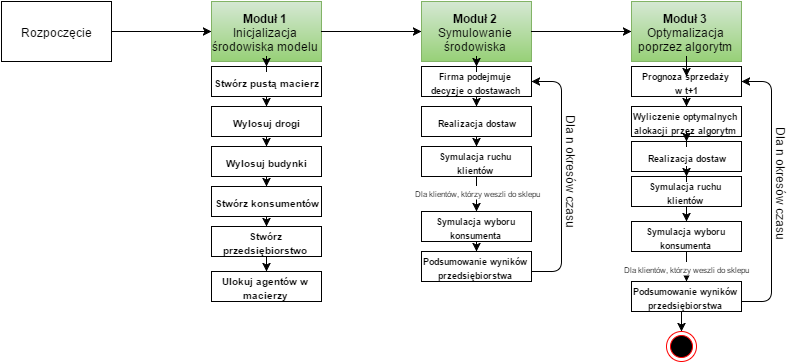
\includegraphics[width=\textwidth]{pictures/Struktura.png}
  \end{subfigure}
  \captionsetup{margin=10pt,font=small,labelfont=bf,width=.8\textwidth}
  \caption[Struktura działania programu]{Podglądowa struktura działania programu. \textit{Źródło:} opracowanie własne.}\label{fig:struktura}
\end{figure}
% --- figure --------------------------------------------------------


\subsection{Generowanie środowiska modelu}
\paragraph{Klasa \textit{rynek}}\mbox{}\\
Za reprezentację tak opisanego środowiska modelu (zob. rozdział \ref{chapter:koncepcja}) odpowiada klasa \textit{rynek}, wobec której dziedziczą wszystkie inne klasy występujące w modelu. Klasa \textit{rynek} (i wszystkie dziedziczące) jest generowana dynamicznie i losowo \footnote{Jednak może być zapisana jeśli istnieje konieczność replikacji obliczeń albo porównań.}.  Konstrukcja klasy \textit{rynek} w programie została zaprezentowana w diagramie \ref{UML:rynek}. \\


% --- figure --------------------------------------------------------
\begin{figure}[hbt]
  \centering
\begin{tikzpicture} \label{rynek}
\begin{class}[text width=11cm]{rynek}{0,0}
\attribute{swiat : class}
\attribute{symulowana\_firma : class}
\attribute{tura : integer}
\attribute{produkty\_na\_rynku : class}
\operation{\_\_init\_\_(self,swiat) : None}
\operation{sprzedaz\_w\_sklepach(self) : None}
\operation{nowatura (self) : None}
\end{class}
\end{tikzpicture}
  \captionsetup{margin=10pt,font=small,labelfont=bf,width=.8\textwidth}
  \caption[Diagram UML klasy rynek]{Diagram UML klasy \textit{rynek} \textit{Źródło:} opracowanie własne.} \label{UML:rynek}
\end{figure}
% --- figure --------------------------------------------------------


\paragraph{Klasa \textit{świat}}\mbox{}\\

Klasa \textit{swiat} zawarta w klasie \textit{rynek} i zaprezentowana na diagramie \ref{UML:swiat} powstała w celu odpowiedniego odwzorowania kluczowego aspektu lokalizacji i dróg w łańcuchach dostaw, wzorując się na podejściu zastosowanym w \textit{modelu segregacji Schellinga} (\cite{Schelling1971}). Agenci osadzeni są w przestrzeni, reprezentowanej przez macierz klas \textit{lokalizacja} o wymiarach (x,y). Dodatkowo, lokalizacje są połączone drogami, wymusząjąc na agentach poruszanie się tylko w obrębie ścieżek. Dzięki temu, w modelu będziemy mogli wiernie odwzorować wpływ odległości i wyboru trasy na efektywność procesów logistycznych, oraz zależność wyników sklepu od zamieszkującej okolicę populacji. 

Macierz \textit{mapa} generowana jest według algorytmu, który gwarantuje, że tak otrzymana mapa środowiska będzie spełniać warunki przedstawione w tabeli \ref{tab:warunki_drogi}. Przykładowa \textit{mapa} otrzymana w wyniku działania algorytmu widoczna jest na rysunku \ref{fig:mapa}.

\begin{table}[hbt]
  \centering
  \captionsetup{margin=10pt,font=small,labelfont=bf,width=.8\textwidth}
  \caption[Warunki generowania mapy środowiska]{Warunki generowania mapy środowiska. \textit{Źródło:} opracowanie własne.}
  \label{tab:warunki_drogi}
\vspace*{2ex}
  \begin{tabular}{ll}
    l.p        & Warunek  \\ \hline
    1     &   Drogi krzyżują się i skręcają tylko pod kątem prostym  \\
    2        &    Poza skrzyżowaniami, drogi nie mają w sąsiedztwie innych dróg     \\
    3 &   Budynki mogą występować tylko w bezpośrednim sąsiedztwie drogi \\ 
    4 &   Drogi stanowią ciągłą linię (nie ma drogi, do której nie można dojechać ) \\ 
    5 &   2 punkty od skraju mapy nie są generowane ani drogi, ani lokalizacje.\footnote{Jest to zabezpieczenie algorytmu, który w odległości 2 pkt od skraju mapy ma 0 proc. szansy na poprowadzenie ścieżki dalej --- ponieważ w przypadku iterowania na skrajach mapy niektóre funkcje (jak sprawdzenie sąsiadujących punktów) mogą odnieść się do lokalizacji poza macierzą, powodując błąd programu.}\\ 
    6 &   Budynki mogą występować tylko w bezpośrednim sąsiedztwie drogi \\   \hline
  \end{tabular}
\end{table}

% --- figure --------------------------------------------------------
\begin{figure}[hbt]
  \centering
\begin{tikzpicture}
\begin{class}[text width=11cm]{swiat}{-1,0}
\attribute{mapa : array \textit{--- macierz lokalizacji o wymiarach x,y}}
\attribute{ludnosc : array type \textit{--- macierz instacj klasy konsument}}
\attribute{ludnosc : dictionary \textit{--- slownik sieci drog}}
\end{class}
\begin{class}[text width=7cm]{lokalizacja}{-5,-5}
\inherit{swiat}
\attribute{typ : string \textit{--- typ budynkui}}
\attribute{x : integer \textit{--- lokalizacja x}}
\attribute{y : integer  \textit{--- lokalizacja y}}
\attribute{droga : array \textit{--- przylegla droga}}
\end{class}
\begin{class}[text width=7cm]{konsument}{3,-5}
\inherit{swiat}
\attribute{plec : string}
\attribute{wiek : integer}
\attribute{zarobki : integer}
\attribute{zainteresowania : array}
\attribute{wyksztalcenie : integer}
\attribute{okazja : boolean}
\attribute{domx : integer}
\attribute{domy : integer}
\attribute{pracax : integer}
\attribute{pracay : integer}
\operation{odwiedzony\_sklep(self,swiat) : None}
\operation{macierz\_cech(self) : array}
\end{class}
\end{tikzpicture}
  \captionsetup{margin=10pt,font=small,labelfont=bf,width=.8\textwidth}
  \caption[Diagram UML klasy swiat, lokalizacja i konsument]{Diagram UML klasy swiat, lokalizacja i konsument \textit{Źródło:} opracowanie własne.}\label{UML:swiat}
\end{figure}
% --- figure --------------------------------------------------------

% --- figure --------------------------------------------------------
\begin{figure}[hbt]
  \centering
  \begin{subfigure}[t]{0.45\textwidth}
    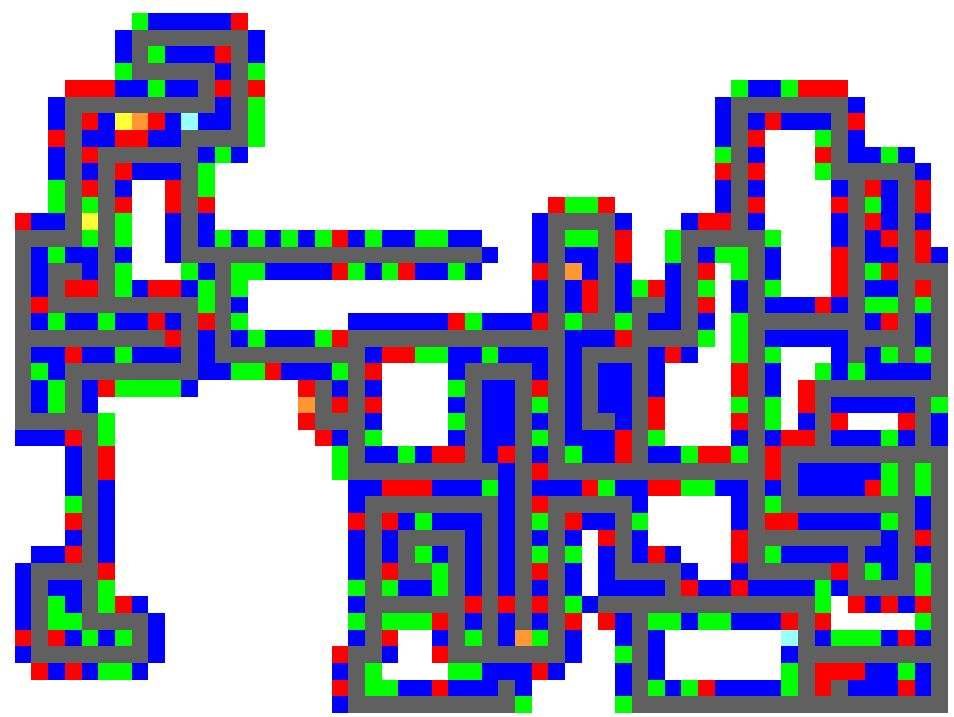
\includegraphics[width=\textwidth]{pictures/mapatypow.png}
  \end{subfigure}
  \captionsetup{margin=10pt,font=small,labelfont=bf,width=.8\textwidth}
  \caption[Przykładowa wygenerowana mapa]{Przykładowa mapa --- \textit{szary} to drogi, \textit{niebieski} --- domy mieszkalne, \textit{czerwony} i \textit{zielony} --- biurowce, \textit{pomarańczowy} --- sklepy, \textit{żółty} --- magazyny, \textit{błękitny} --- fabryki \textit{Źródło:} opracowanie własne.}\label{fig:mapa}
\end{figure}
% --- figure --------------------------------------------------------


Trasy pomiędzy zadanymi punktami w modelu są wyszukiwane dynamicznie, na podstawie algorytmu wyszukiwania drogi. Odległości z kolei obliczane są poprzez sumowanie ilości punktów w zwracanym przez algorytm łańcuchu. 

Algorytm oparty jest na metodach wyszukiwania ścieżek w grafach, dzięki założeniu, że każda droga o współrzędnej $(x,y)$ na mapie jest punktem grafu, który może sąsiadować z punktami o współrzędnych $(x-1,y),(x+1,y),(x,y+1),(x,y-1)$ \footnote{Punkty $(x-1,y-1),(x+1,y-1),(x+1,y+1),(x-1,y+1)$ wykluczamy przez wcześniejsze założenie, że drogi krzyżują się tylko pod katem prostym.}, o ile również są drogrami. \footnote{Informacje o punktach i sąsiadujących przechowywane są w zmiennej nodes, która jesst słownikiem, dla każdego klucza --- punktu na mapie --- przechowuje informacje o sąsiadujących punktach, np. $(3,2) = [(3,3)(4,3)]$.} \footnote{Pewnym ograniczeniem jest, że jako punkty grafu definiujemy tylko drogi, tak więc szukając trasy z punktu A do punktu B, de facto szukamy trasy z drogi przy punkcie A do drogi przy punkcie B.}

Algorytm, udostępniony przez Python Foundation \footnote{https://www.python.org/doc/essays/graphs/} i zaprezentowany w tabeli \ref{fig:wayfinding} ma następujące cechy
	\begin{itemize}
		\item jest rekurencyjny,
		\item nie jest losowy,
		\item nie gwarantuje znalezienia najkrótszej trasy.
	\end{itemize}


% --- figure --------------------------------------------------------
\begin{figure}[hbt]
  \centering
\begin{lstlisting}[frame=single, label=szukaniedrogi]  
    def find_path(graph, start, end, path=[]):
        path = path + [start]
        if start == end:
            return path
        if not graph.has_key(start):
            return None
        for node in graph[start]:
            if node not in path:
                newpath = find_path(graph, node, end, path)
                if newpath: return newpath
        return None
\end{lstlisting}
  \captionsetup{margin=10pt,font=small,labelfont=bf,width=.8\textwidth}
  \caption[Algorytm wyszukiwania drogi]{Algorytm wyszukiwania drogi \textit{Źródło:} opracowanie własne.}\label{fig:wayfinding}
\end{figure}
% --- figure --------------------------------------------------------


\subsection{Agenci, ich rodzaje i właściwości}
\subsubsection{Konsumenci} \label{chapter:konsumenci}

Idąc za \cite{Kaminski2012}, w modelu stosujemy modelowanie rynku za pomocą heterogenicznych konsumentów. Stąd, każdy z konsumentów ma swoją unikalną charakterystykę rozumianą przez cechy demograficzne oraz cechy charakteru, które będą wpływać na jego wybory. 

Aspekt lokalizacji i ruchu agenta jest symulowane zgodnie z opisem zawartym w rozdziale \ref{chapter:koncepcja}. Warto zwrócić uwagę na to, że chociaż agenci nieustannie poruszają się w ramach modelu, to pula lokalizacji w ramach których będą się przemieszczać jest ograniczona. Każdy z konsumentów będzie się przemieszczał tylko w wyniku predefiniowanych zdarzeń, których liczba dla każdego konsumenta jest ograniczona do czterech \footnote{Warto zauważyć, że każde ze zdarzeń wywołuje przemieszczenie do korespondującej lokalizacji, tak zdarzenie będzie zawsze wywoływać podróże tej samej lokacji}, tak więc agent będzie przemieszczał się pomiędzy maksymalnie czterami lokalizacjami, tworząc pewne wzorce zachowań. 

Dzięki temu, odwzierciedlamy zjawisko ze świata rzeczywistego, że konsumenci zazwyczaj robią zakupy w ograniczonej liczbie sklepów będących po drodze bądz niedaleko. Jest to bardzo istotny warunek funkcjonowania modelu, ponieważ losowy dobór klientów uniemożliwiłby modelowanie predykcyjne.


% --- figure --------------------------------------------------------
\begin{figure}[hbt]
  \centering
\begin{tikzpicture}
\begin{class}[text width=11cm]{konsument}{0,0}
\attribute{plec : string}
\attribute{wiek : integer}
\attribute{zarobki : integer}
\attribute{zainteresowania : array}
\attribute{wyksztalcenie : integer}
\attribute{okazja : boolean \textit{--- wskazanie powodu wyjścia z domu}}
\attribute{domx : integer \textit{--- współrzędna x domu}}
\attribute{domy : integer \textit{--- współrzędna y domu}}
\attribute{pracax : integer \textit{--- współrzędna x pracy}}
\attribute{pracay : integer \textit{--- współrzędna y pracy}}
\operation{odwiedzony\_sklep(self,swiat) : None}
\operation{macierz\_cech(self) : array}
\end{class}
\end{tikzpicture}
  \captionsetup{margin=10pt,font=small,labelfont=bf,width=.8\textwidth}
  \caption[Diagram UML klasy konsument]{Diagram UML klasykonsument \textit{Źródło:} opracowanie własne.}\label{UML:konsument}
\end{figure}
% --- figure --------------------------------------------------------

Każdy będzie definiowany w klasie o właściwościach zdefionowanych w diagramie \ref{UML:konsument}. Wartości cech dla każdego z konsumentów są losowane na podstawie rozkładów publikowanych przez Główny Urząd Statystyczny \cite{GUS2011} oraz danych firmy Sedlak\&Sedlak (\cite{Sedlak2013}) \footnote{Raporty firmy Sedlak\&Seldlak służyły do zbudowania tabeli prawdopodobieństwa wystąpienia danego wynagrodzenia w zależności od płci i wykształcenia. Reszta danych oparta na GUS} w celu zagwarantowania odzwierciedlenia struktury społeczeństwa. Ze względu na zastosowanie prawdopodobieństw warunkowych dla niektórych cech (np. zarobki są zależne od wcześniej wylosowanego wykształcenia) istnieje pomiędzy nimi korelacja. Przykładowe rozkłady pokazane są na rysunku \ref{fig:wiek} oraz \ref{fig:wyksztalcenie}.

Poza zaprezentowanymi na histogramach danymi demograficznymi agenci posiadają zainteresowania określone zmiennymi binarnymi. W przeciwieństwie do danych demograficznych, są one niezależne, a każda z nich posiada identyczną szansę na wylosowanie. Celem ich wprowadzenia było stworzenie zmiennych, których nie byłyby skorelowane z danymi demograficznymi. Ponieważ mają wpływ na wybory klientów i nie są zapisywane w historii transakcji \footnote{W przeciwieństwie do danych demograficznych (wiek, wykształcenie, płeć) nie są znane przedsiebiorstwu w modelu i dlatego nie są zapisywane w historii transakcji.}, utrudniają przewidywanie sprzedaży.

% --- figure --------------------------------------------------------
\begin{figure}[hbt]
  \centering
  \begin{subfigure}[t]{0.45\textwidth}
    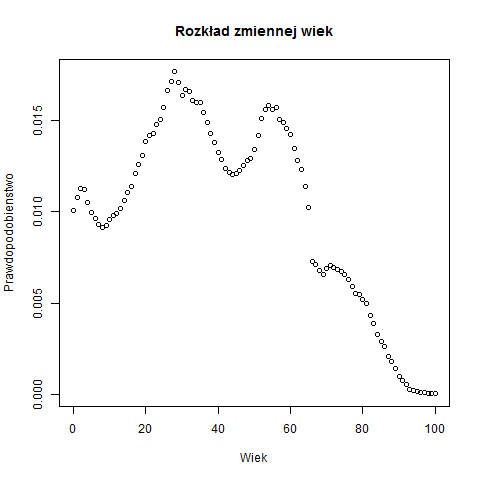
\includegraphics[width=\textwidth]{pictures/wiek.png}
    \caption{Rozkład prawdopodobieństwa zmiennej wiek}
    \label{fig:wiek}
  \end{subfigure}
  \hfill
  \begin{subfigure}[t]{0.45\textwidth}
    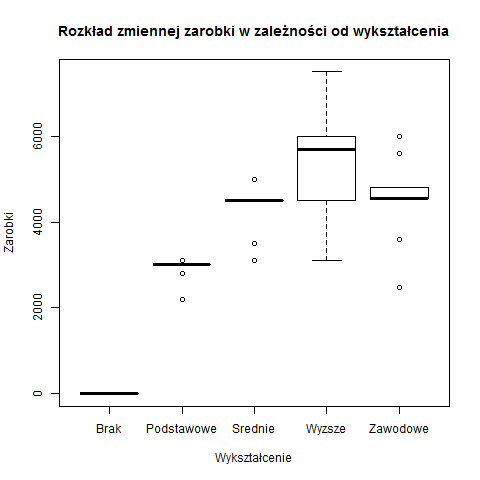
\includegraphics[width=\textwidth]{pictures/wyksztalcenie_zarobki.png}
    \caption{Rozkład prawdopodobieństwa zmiennej wykształcenie}
    \label{fig:wyksztalcenie}
  \end{subfigure}
  \captionsetup{margin=10pt,font=small,labelfont=bf,width=.8\textwidth}
  \caption[Rozkłady zmiennych cech klasy konsument]{Rozkłady zmiennych cech klasy konsument \textit{Źródło:} opracowanie własne na podstawie danych Narodowego Spisu Ludności 2011, \cite{GUS2011}.}\label{fig:cechykonsumenta}
\end{figure}
% --- figure --------------------------------------------------------


\subsubsection{Przedsiębiorstwo}

Zgodnie z założeniami określonymi w rozdziale 1, symulowane przedsiębiorstwo jest zbiorem elementów. Zbiór ten należy w modelu do klasy \textit{firma}, przechowującej w macierzach instancje klas \textit{fabryka, magazyn, sklep}, jak zaprezentowano na diagramie \ref{UML:firma}. W klasie \textit{firma} znajdują się także funkcje przynależne opisywanemu w strukturze modelu zarządowi, mające na celu koordynację działania przedsiębiorstwa. 

Warto zauważyć, że klasy te mają wiele wspólnych właściwości, z wyjątkami obecnymi w klasie \textit{sklep}. Wynika to z konieczności stworzenia funkcji symulujących procesy sprzedażowe oraz faktu, że sklepy mają dodatkowe zmienne przechowujące informacje o składzie towaru, klientach odwiedzających sklep w danej jednostce czasu $t$ oraz historii transakcji.  

% --- figure --------------------------------------------------------
\begin{figure}[hbt]
  \centering
\begin{tikzpicture} \label{firma}
\begin{class}[text width=7cm]{firma}{-1,0}
\attribute{fabryki : array}
\attribute{magazyny : array}
\attribute{sklepy : array}
\attribute{produkt : array}
\attribute{cena : array}
\operation{klienci\_w\_sklepach(self,swiat,tura)}
\operation{przypisz\_koszty(self,losowe,skala)}
\end{class}
\begin{class}[text width=6cm]{fabryka magazyn}{-5,-7}
\inherit{firma}
\attribute{nazwa : string}
\attribute{lokalizacja : array}
\attribute{oblozenie : integer}
\attribute{koszt : integer}
\attribute{efekt\_skali : integer}
\attribute{symbol : sympy.symbol}
\end{class}
\begin{class}[text width=7cm]{sklep}{2,-7}
\inherit{firma}
\attribute{nazwa : string}
\attribute{lokalizacja : array}
\attribute{oblozenie : integer}
\attribute{koszt : integer}
\attribute{efekt\_skali : integer}
\attribute{symbol:sympy.symbol}
\attribute{klienci : array}
\attribute{klienci\_historycznie : array}
\attribute{sklad : dictionary}
\attribute{sprzedaz : array}
\attribute{przewidywana\_sprzedaz:integer}
\operation{dostawa\_towaru(self, rynek, trasa, ilosc)}
\operation{sprzedaz\_w\_sklepie(self, towar)}
\end{class}
\end{tikzpicture}
  \captionsetup{margin=10pt,font=small,labelfont=bf,width=.8\textwidth}
  \caption[Diagram UML klasy firma, fabryka, magazyn oraz sklep]{Diagram UML klasy firma, fabryka, magazyn oraz sklep \textit{Źródło:} opracowanie własne.}\label{UML:firma}
\end{figure}
% --- figure --------------------------------------------------------

\subsubsection{Produkt} \label{chapter:produkt}

Jak zauważa \cite{Sagan2011}, który wskazuje na istnienie nurtu w dziedzinie modelowania strukturalnego zachowań klientów, które wykorzystywało zmienne marketingowe określające jakość produktu i liczbę cech \footnote{Mowa o tzw. nurcie poznawczym albo nurcie teorii przetwarzania informacji --- TPI}. Opierając się tej obserwacji zakładamy, że każdy produkt charakteryzuje się cechami wpływające na prawdopodobieństwo jego zakupu przez konsumentów które mogą być wyrażone ilościowo. 

\paragraph{Piwo jako symulowany produkt}\mbox{}\\

Dlatego w modelu produkt definiujemy przez zestaw wybranych cech które odróżniają go od produktów konkurencji, które mogą przyjąć formę skali ocen, zmiennych binarnych bądź zmiennych kategorycznych. \footnote{Ich istotność nie jest w tym momencie ważna, ponieważ nawet jeśli w zbiorze znajdzie się cecha mająca mały wpływ na decyzje konsumentów, zostanie ona wyeliminowana na etapie tworzenia modelu bądź drzewa klasyfikacyjnego ze względu brak istotności statystycznej współczynnika}, a klasa \textit{produkt} przechowujące jednowymiarową macierz z cechami produktu.

Warto odnotować, że w pracy przyjmujemy, że symulowanym produktem z branży FMCG jest piwo. Ten dość nieelegancki wybór motywowany jest głównie specyfiką produktu, która dobrze pasuje do wymagań stawianych przez model (szczególnie w aspekcie możliwości modelowania decyzji konsumenckich), wśród których należy zwrócić uwagę na:

	\begin{itemize}
			\item Wysoka sprzedaż i idący za tym wysoki obrót towaru w sklepach. Przeciętny polak pije 99 litrów piwa rocznie, co oznacza butelkę kupioną co mniej więcej drugi dzień. Dzięki temu możemy założyć, że prawdopodobieństwo zakupu piwa przez klienta to nawet 50\% , a to z kolei gwarantuje odpowiednią liczbę iteracji do przeprowadzenia symulacji. 
			\item Piwa mają silne marki o ugruntowanych cechach i grupach docelowych --- reklamy piw zazwyczaj kierowane są do precyzyjne określonych grup docelowych, co powoduje, że występuje wysoka zależność pomiędzy charakterystyką demograficzną klienta a piwem które wybierze, \footnote{Idealnym przykładem jest Redd's, wybierany głównie przez kobiety. Innymi mogą być Grolsch wybierany przez ludzi zamożnych, kiedy Wojak trafia do najgorzej zarabiających.}.  Przykładowo, piwo smakowe i pszeniczne będą trafiać do dwóch różnych grup klientów.
	\end{itemize}

% --- figure --------------------------------------------------------
\begin{table}[hbt]
  \centering
  \captionsetup{margin=10pt,font=small,labelfont=bf,width=.8\textwidth}
  \caption[Cechy charakteryzujące produkt w modelu]{Cechy charakteryzujące produkt w modelu. \textit{Źródło:} opracowanie własne.}
  \label{tab:cechyproduktu}
\vspace*{2ex}
\begin{tabular}{llll}
\hline
Cecha       & Skala & Opis                                                                                                        \\ \hline
Cena        & 1-5   & Relatywna cena produktu                                                             \\
Smak        & 1-5   & Relatywna jakość smaku produktu                                                       \\
Opakowanie  & 1-5   & Relatywna atrakcyjność opakowania produktu                                           \\
Premium      & 0-1   & Czy produkt jest postrzegany jako marka premium? \\
Budżetowy   & 0-1   & Czy produkt jest postrzegany jako marka budżetowa?  \\
Lager        & 0-1   & Czy produkt należy do piw typu lager?                                                                       \\
Smakowe     & 0-1   & Czy produkt należy do piw smakowych?                                                                        \\
Marketing   & 0-5   & Wysokość nakładów na marketing marki                                                                        \\ \hline
\end{tabular}
\end{table}
% --- figure --------------------------------------------------------

\subsubsection{Konkurencja}
 
W założeniach przyjmujemy, że konkurencja jest pasywna, tj. nie podejmuje działań ani decyzji w trakcie trwania symulacji. Wynika to z odmiennego celu badania, którym jest analiza działania algorytmów optymalizacyjnych. Nagłe zmiany sprzedaży spowodowane np. obniżeniem ceny przez konkurencję spowodowałyby wątpliwości interpretacyjne i są zbędne. Konkurencja jest za to potrzebna do stworzenia alternatywnych dla symulowanego produktu, o odmiennych cechach i przyciągających klientów o specyficznych charakterystykach, i jej rola ogranicza się do wprowadzenia go na rynek oraz zapewnienie dostaw do każdego ze sklepów.

\subsubsection{Ścieżki i trasy dostaw}

Klasa \textit{trasy} przechowuje wszystkie możliwe kombinacje elementów grafu (ścieżki), zdefiniowanych w rozdziale \ref{chapter:zadanie}, składające się z instacji klas \textit{fabryka}, \textit{magazyn}, \textit{sklep} oraz \textit{krawędzi} pomiędzy nimi \footnote{Jako ścieżkę rozumiemy sekwencję punktów z drogami, jakie trzeba przebyć od fabryki do magazynu i od magazynu do sklepu.}. W przypadku złożonych grafów (czyli sytuacji, kiedy przedsiębiorstwo składa się z wielu jednostek) liczba kombinacji może uniemożliwić swobodne przetwarzanie klasy w pamięci komputera, jednak w takim wypadku można predefiniować zbiór możliwych łańcuchów, spośród których model będzie wybierał najbardziej optymalne trasy (zob. rozdział \ref{chapter:cechy}).

Dla każdej z tras, poza informacjami o jednostkach wchodzących w skład przedsiębiorstwa, przechowujemy także informację o \textit{scieżkach} pomiędzy jednostkami. Wynika to z faktu, że transporty pomiędzy poszczególnymi jednostkami także mogą doświadczać efektów skali, \footnote{Przykładowo, pod kątem kosztów na produkt, transport 100 produktów może być bardziej opłacalny niż 10 ze względu na rozłożenie kosztów stałych na większą ilość produktów.} a długość ścieżki bezpośrednio wpływa na koszt łańcucha --- koszt wzrasta wraz z długością ścieżki.

\subsection{Symulowanie decyzji konsumenckich} \label{chapter:customerresearch}

Jak wskazano na diagramie \ref{fig:struktura}, podczas wizyty każdego z wirtualnych konsumentów w sklepie symulujemy jego decyzję co do zakupu towaru. Naszą intencją jest, aby decyzje konsumentów w modelu jak najbardziej przypominały decyzje klientów w analogicznych sytuacjach w świecie rzeczywistym \footnote{Warto odnotować, że to nie jest to samo co późniejsze przewidywanie "prognozowanej sprzedaży".}.

Opierając się na \cite{Sagan2011} (zob. rozdział \ref{chapter:produkt}), wiemy, że jesteśmy w stanie zdefiniować kluczowe cechy konsumenta i cechy marketingowe produktu jako zbiór zmiennych ilościowych. Wykorzystując to stwierdzenie, w grze eksperymentalnej przeprowadzonej na potrzeby pracy \footnote{Gra dostępna jest pod adresem http://serwer1418288.home.pl/test/piwo/zapisy.php}, poproszono uczestników o stwierdzenie, jakie produkty z dostępnej listy kupi klient o charakterystyce wylosowanej przez program. Po odpowiedzi udzielonej przez gracza, predefiniowane, jakościowe cechy produktu były transponowane na wartości liczbowe \footnote{Produkty obecne w ankiecie należą do jednego z większych koncernów browarniczych, a w celu zapewnienia realistycznego oddania cech produktów i preferencji klientów konstrukcja gry ekonomicznej była konsultowana z pracownikami wspomnianego koncernu.}\footnote{Na przykład, piwo Grolsh jest drogie, klasy premium i jest lager, stąd otrzyma zapis [5,1,1], a tani smakowy Redd's [3,0,0].} i wraz z ilościowymi cechami klienta oraz zmienną binarną przechowującą informacje \textit{kupił/niekupił} zapisywany na serwerze SQL. 

W programie dane te służą do budowy drzewa klasyfikacyjnego, które --- ponieważ dane cech agentów oraz dane z gry ekonomicznej są w identycznej formie --- dla każdej kwerendy o klienta i produkt zwraca prawdopodobieństwo zakupu. Dla każdego agenta możemy zbudować listę prawdopodobieństw zakupu każdego z towarów dostępnego na rynku. Zastosowane podejście gwarantuje wysokie podobieństwo z wyborami realnych konsumentów ze względu na:

	\begin{itemize}
		\item wysoką liczbą rekordów istnieje duże prawdopodobieństwo, że istnieje zapis o decyzjach klienta o bardzo podobnej charakterystyce,
		\item baza danych jest generowania przez decyzje ludzkie, zapewniając wysoką zgodność z analogicznymi wyborami w świecie rzeczywistym,
		\item wybór drzewa klasyfikacyjnego  jako metody i duża ilość danych użytych do jego stworzenia, pozwala na bardzo bardzo dokładne odwzorowane zbioru uczącego, które \cite{James2013} określa jako \textit{overfit}. 
	\end{itemize}

% --- chapter ---------------------------------------------------------
\clearpage
\section{Efekty działania algorytmu optymalizacyjnego}

Proponowany algorytm został zaimplementowany do modelu wieloagentowego symulującego przedsiębiorstwo i rynek. Wyniki działania algorytmu sugerują, że jego zastosowanie w przedsiębiorstwach pozwala na zwiększenie rentowności przez dostosowanie wolumenu dostaw do popytu w każdym ze sklepów, oraz minimalizacji kosztów dostaw.

\subsection{Założenia modelu}

Weryfikacja działania algorytmu odbywać się będzie w modelu stworzonym zgodnie z założeniami opisanymi w rozdziale \ref{chapter:koncepcja}, w oparciu o losowo wygenerowane środowisko działania modelu (\textit{świat i rynek}). Właściwości środowiska modelu zostały opisane zostały opisane w w tabeli \ref{tab:zalozenia}, a \textit{mapy} powstałego w ten sposób środowiska zostały przedstawione na wykresach \ref{symulowanamapa} i \ref{symulowanaludnosc}.

\begin{table}[hbt] 
  \centering
  \captionsetup{margin=10pt,font=small,labelfont=bf,width=.8\textwidth}
  \caption[Właściwości generowanego świata]{Założenia generowanego świata. \textit{Źródło:} opracowanie własne.}
  \label{tab:zalozenia}
\vspace*{2ex}
  \begin{tabular}{lccc}
    Właściwość        & Założenie \\ \hline
    Populacja & $2 500$\\
    Wymiar $x$ & $60$\\
    Wymiar $y$ & $60$\\ 
    Udział dróg & $0.3$\\ 
    Gęstość zakrętów dróg & $0.05$\\  
    Udział budynków mieszkalnych & $0.6$\\  
    Udział biurowców \footnote{Biurowce są dla konsumentów miejscem pracy, do których podróżują codziennie} & $0.2$\\  
    Udział przestrzeni komercyjnej \footnote{Przestrzeń komercyjna to miejsca, w którym można założyć sklep, fabrykę bądź magazyn, tak więc razem tworzą zbiór miejsc gdzie przedsiębiorstwo może losowo wygenerować swoją jednostkę}& $0.2$\\  \hline
    Ilość fabryk & $2$\\ 
    Ilość magazynów & $2$\\ 
    Ilość ilość sklepów & $4$\\ 
    Cena produktu & $7$\\ 
  \end{tabular}
\end{table}

\begin{figure}[hbt]
  \centering
  \begin{subfigure}[t]{0.45\textwidth}
    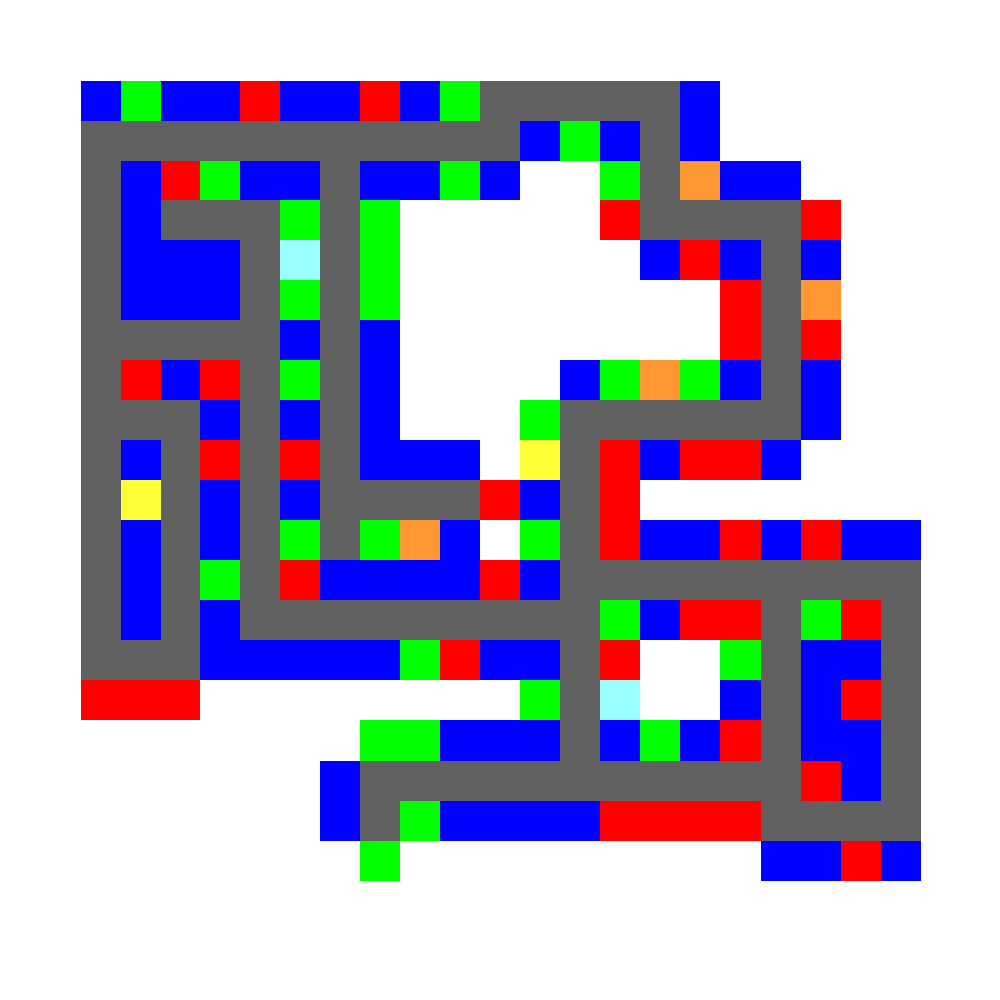
\includegraphics[width=\textwidth]{../mapy/typy.png}
    \caption{Mapa typów lokacji na mapie}
    \label{symulowanamapa}
  \end{subfigure}
  \hfill
  \begin{subfigure}[t]{0.45\textwidth}
    
\includegraphics[width=\textwidth]{../mapy/ludnosc.png}
    \caption{Histogram występowania konsumentów na mapie.}
    \label{symulowanaludnosc}
  \end{subfigure}
  
  \captionsetup{margin=10pt,font=small,labelfont=bf,width=.8\textwidth}

  \caption[Wygenerowane mapy środowiska modelu ]{Wygenerowane mapy środowiska modelu. \textit{Źródło:} opracowanie własne.}\label{fig:generowanemapy}
\end{figure}

\paragraph{Konsumenci}\mbox{}\\
Cechy konsumentów zostały wygenerowane zgodnie z rozkładami zawartymi w Narodowym Spisie Ludności (\cite{GUS2011}) oraz XI Ogólnopolskim Badaniu Wynagrodzień \cite{Sedlak2013} w celu zapewnienia spójności z rzeczywistą strukturą społeczną. Przykładowe histogramy cech klientów w rozważanym modelu zostały zaprezentowane na wykresie \ref{ludnosc}. 

Jak zostało opisane w rozdziale \ref{chapter:konsumenci}, cechy klientów wpływają na ich decyzji konsumenckie i wybór produktów w sklepie. Dlatego profil klienta konsumującego symulowany produkt (zob. tabela \ref{tab:produkty}) będzie dystynktywny, tak jak w normalnych warunkach rynków różne marki przyciągają klientów o różnych profilach i cechach demograficznych. Właściwość tą wykorzystujemy do modelowania predyktywnego prawdopodobieństwa zakupu przy danej charakterystyce klienta w czasie $t+1$. Porównanie rozkładów cech ogółu klientów i konsumentów marki zaprezentowano na wykresie \ref{profile}.



\paragraph{Przedsiębiorstwo}\mbox{}\\
Symulowane przedsiębiorstwo, zdefiniowane jak w rozdziale \ref{chapter:zadanie}, zostało wygenerowane zgodnie z założeniami przedstawionymi w tabeli \ref{tab:zalozenia}. Składa się z 2 fabryk, 2 magazynów i 4 sklepów, które wspólnie tworzą  $2\choose 1 $ $ \times $ $2\choose 1 $ $ \times $ $4\choose 1 $ = 16 możliwych ścieżek $w$ (zob. rozdział \ref{chapter:zadanie}). Lokalizacje poszczególnych jednostek przedsiębiorstwa zostały zaprezentowane na rysunku \ref{mapafirma}.

Jak opisanano w rozdziale \ref{chapter:koncepcja}, każdy z $j$ elementów przedsiębiorstwa oraz krawędzie $d$ je łączące powiązane jest z funkcją kosztu $f_j$, które w celu symulacji efektów skali są nieliniowe. Dla fabryk, magazynów i sklepów zakładamy ujemne korzyści skali, podczas gdy dla transportu na krawędziach --- dodatnie. Dokładne funkcje kosztów wykorzystane w modelu opisane są w tabeli \ref{tab:funkcje_kosztow}. 

\begin{table}[hbt]
  \centering
  \captionsetup{margin=10pt,font=small,labelfont=bf,width=.8\textwidth}
  \caption[Założone w modelu funkcje kosztów]{Założone w modelu funkcje kosztów. \textit{Źródło:} opracowanie własne.}
  \label{tab:funkcje_kosztow}
\vspace*{2ex}
  \begin{tabular}{lccc}
    Jednostka        & Symbol & Funkcja kosztu \footnote{$x_j$ definiujemy jako wolumen przechodzący przez dany element grafu $f \in S$}\\ \hline
    Fabryka    & $fa \in FA$   &    $f_{fa} =  1.3 \times x_{fa} ^{1.03}$ \\
    Magazyn & $ma \in MA$  & $ f_{ma} = 1.2 \times x_{ma} ^{1.05}$\\
    Sklep & $sk \in SK$ & $f_{sk} = 1.1 \times x_{sk} ^{1.07}$\\ 
    Droga (krawędź ) & $ d \in D \footnote{$l_d$ jest długością krawędzi, liczoną jako ilość punktów które należy przebyć od jej początku do końca}$ & $ f_{d} = 0.005 \times l_d \times x_{d} ^{0.95}  $ \\ \hline
  \end{tabular}
\end{table}

\paragraph{Produkty}\mbox{}\\
W modelu zakładamy, że na rynku obecnych jest 7 marek piwa, z których jedno należy do symulowanego przez nas przedsiębiorstwa (produkt o nazwie \textbf{Symulowane}). Jak opisano w rozdziale \ref{chapter:produkt}, każde z piw zdefiniowane jest 7 zmiennymi marketingowymi, których wartości zostały wylosowane dla każdego z produktów na rynku. Cechy produktów zostały zaprezentowane zostały w tabeli \ref{tab:produkty}. Wyniki sprzedaży poszczególnych marek w jednostkach czasu $t$ zaprezentowane są na wykresie \ref{fig:sprzedaz_marek}.

Analiza wyników sprzedaży oraz cech produktu symulowanego przedsiębiorstwa pozwala zauważyć (zob. wykres \ref{fig:sprzedaz_marek}, tabela \ref{tab:produkty}), że piwo należące do symulowanego przez nas przedsiębiorstwa należy do jednych z najtańszych piw na rynku, jest piwem smakowym o przeciętnych walorach smakowych, ale za to intensywnych nakładach na marketing i dużej uwadze poświęconej projektowaniu opakowania. Skonfrontowanie tego z profilem klienta widocznym na wykresie \ref{profile} pozwala zrozumieć, dlaczego nabywcy naszego piwa należą do grupy gorzej sytuowanych finansowo, raczej młodszych \footnote{Wynika to z połączenia faktów, że młode osoby mniej zarabiają, oraz piwa smakowe nie są zbyt popularne wsród starszych roczników}, z dominującą grupą kobiet. Profil wykształcenia nie różni się znacząco od przeciętnej, z delikatnie mniejszym udziałem klientów o wyższym wykształceniu.



\begin{table}[hbt] 
  \centering
  \captionsetup{margin=10pt,font=small,labelfont=bf,width=.8\textwidth}
  \caption[Cechy symulowanych produktów]{Cechy symulowanych produktów. \footnote{Cechy określone przez nazwy binarne zostały opisane skrótem: P --- premium, B --- budżetowe, L --- lager, S --- smakowe} \footnote{Opis poszczególnych cech zawarty jest w tabeli \ref{tab:cechyprodukty}}\textit{Źródło:} opracowanie własne.}
  \label{tab:produkty}
\vspace*{2ex}
  \begin{tabular}{rcccccccc}
  \hline
 & Cena & Smak & Opakowanie & P & B & L & S & Marketing \\ 
  \hline
\textbf{Symulowane} &   1 &   3 &   5 &   0 &   0 &   0 &   1 &   4 \\ 
  Slaskie &   4 &   4 &   2 &   1 &   0 &   1 &   0 &   4 \\ 
  Lebskie &   4 &   2 &   2 &   1 &   0 &   0 &   1 &   5 \\ 
  Babskie &   4 &   3 &   5 &   0 &   1 &   0 &   1 &   5 \\ 
  Pszczeniczne &   2 &   2 &   2 &   0 &   0 &   0 &   1 &   2 \\ 
  Opolskie &   4 &   3 &   5 &   0 &   0 &   0 &   1 &   4 \\ 
  Mocne &   4 &   2 &   2 &   1 &   0 &   1 &   0 &   3 \\ 
   \hline
\end{tabular}
\end{table} 



\subsection{Przewidywanie decyzji konsumentów}

Przewidywanie decyzji konsumentów odbywa się zgodnie z założeniami przedstawionymi w rozdziale \ref{chapter:statistical}. \footnote{W modelu stosowane jest pewne uproszczenie podczas prognozowania ilości klientów w sklepie w $t+1$. Ponieważ wizyta klienta w sklepie jest w modelu zdarzeniem losowym (losuje się jedna z czterech lokalizacji docelowych), a model nie symuluje efektów zewnętrznych jak pogoda czy dzień tygodnia, do przewidywania liczby klientów odwiedzających sklep w chwili $t+1$ stosowana jest po prostu średnia z ilośći odwiedzin z poprzednich okresów. Brak jest bowiem zmiennych objaśniających które mogłyby zostać wykorzystane w modelu. Ich wprowadzenie dodawałoby niepotrzebną złożoność do modelu, a zastosowane uproszczenie nie ma wpływu na badanie wyników działania algorytmu.}. Kolejne kroki prognozowania sprzedaży w każdym ze sklepów w czasie $t+1$ to 

\begin{enumerate}
	\item Na podstawie historii transakcji obliczamy średnią ilość klientów $n$ odwiedzających sklep w jednostce czasu $t$,
	\item Na podstawie historii cech klientów kupujących produkt, obliczamy prawdopodobieństwo warunkowe wystąpienia wszystkich zestawów cech, i losujemy cechy dla $n$ klientów w $t+1$ ,
	\item Dla każdego z tak otrzymanych klientów na podstawie przeszłej historii wyborów klientów, wykorzystując metodę regresji logistycznej bądź klasyfikacji $k$-nearest neighbours, obliczamy prawdopodobieństwo zakupu produktu symulowanej firmy,
	\item Kroki 1-3 powtarzamy założoną ilość razy \footnote{W modelu przyjmujemy 3 iteracje prognoz z których obliczana jest średnia.} i obliczamy średnią z trzech obserwacji.
\end{enumerate} 

Analizując wyniki prognozowania, przedstawione na wykresie \ref{fig:prognozy_porowniania} możemy zobserwować ciekawe różnice w skuteczności prognoz obu stosowanych metod --- \textit{regresji logistycznej} oraz \textit{k-nearest neighbours}. Chociaż współczynnik determinacji $R^2$ jest wyższy dla metody regresji logistycznej ($R_{lg}^2 = 0,7912$) niż dla K-nearest neighbours ($R_{kn}^2 = 0,7591$), to ważnym aspektem działania regresji logistycznej jest nie przeszacowywanie sprzedaży (tak jak to robi K-nearest neighbours). Nadmierny optymizm metody K-nearest neighbours powoduje, że algorytm dostarzca do sklepów produkty o których wiemy, że nie zostaną sprzedane. Powoduje to ponoszenie niepotrzebnych koszty produkcji i transportu (zob. wykres \ref{fig:wynikifin}. 

Jak możemy to zaobserwować na wykresie \ref{fig:rozklad_lg_kn}, wynika to z faktu, że K-nearest neighbours dla współczynnika $k=3$ ma większe trudności z jednoznacznym określeniem klasy przewidywanej zmiennej \footnote{Warto przypomnieć, że w tym momencie modelujemy to, czy dany klient będzie w klasie 0 (\textit{nie kupił}) czy 1 (\textit{kupił}).} niż regresja logistyczna. Regresja logistyczna jest o wiele bardziej skłonna to przyporządkowania niskiego prawdopodobieństwa zakupu, jednak z większą pewnością określa klientów którzy kupią produkt. Tymczasem, K-nearest neighbours często wskazuje wartość prawdopodobieństwa w środku przedziału $(0,1)$, co należy interpretować jako odpowiedź niejednoznaczną. Możliwe, że manipulacja współczynnikiem $k$ wpłynęłaby zwracane przez metodę wartości prawdopodobieństwa, jednak w przypadku modelu za bardziej skuteczną będziemy uważać metodę regresji logistycznej. 

\subsection{Wpływ działania algorytmu na działanie przedsiębiorstwo} \label{chapter:wyniki}

Po uruchomieniu programu przez $n=20$ jednostek czasu $t$, przedsiębiorstwo podejmuje decyzje na podstawie predefiniowanych zasad opisanych w rozdziale \ref{chapter:koncepcja} w celu uzyskania punktu odniesienia dla porównania wyników firmy. Po $n=20$ jednostkach czasu, na podstawie dotychczasoo zebranych w modelowanych sklepach historiach transakcji, inicjalizowane są modele regresji logistycznej oraz K-nearest neighbours. Służa one słuzą do prognozowania sprzedaży w każdym ze sklepów w $t+1$. Zgodnie z przyjętymi w rozdziale \ref{chapter:zadanie}, wiedza o sprzedaży w każdym ze sklepów w $t+1$ pozwala nam, po odpowiednich przekształceniach, zbudować algorytm optymalizujący procesy produkcyjno-logistyczne, przede wszystkim pod kątem alokacji wolumenów produkcji i tras dostaw pomiędzy poszczególne jednostki przedsiębiorstwa. 

\paragraph{Alokacje na trasach dostaw (ścieżkach)}\mbox{}\\

W rezultacie działania modelu otrzymujemy wektor $A$, który dla każdego elementu zbioru $w \in W$ (zob. rozdział \ref{chapter:zadanie}) zawiera optymalny \footnote{Zastrzeżenia wobec optymalności alokacji sugerowanych przez algorytm znalazły się w rozdziale \ref{chapter:algorytm}} wolumen dostaw w $t+1$. Wektory otrzymane w toku działania modelu zostały zaprezentowane na w formie wykresu na rysunku \ref{fig:sciezki}.

Obserwując wolumeny dostaw na ścieżkach można zauważyć, że przedsiębiorstwo sterowane przez algorytm jest o wiele bardziej elastyczne co do wyboru ścieżek. Wskazuje wskazuje rosnąca po $t=20$ wariancja wolumenów alokacji na poszczególnych ścieżkach. Ponadto, algorytm wielokrotnie decyduje się dostarczyć towar do sklepu z wielu źródeł. Biorąc pod uwagę, że funkcje kosztów są nieliniowe a we wszystkich jednostkach firmy występują negatywne efekty skali, pozwala to znaczące ograniczenie kosztów, których spadek widoczny jest na wykresie \ref{fig:wynikifin}.

To o tyle istotna obserwacja, że w praktyce biznesowej podobne metody ograniczenia kosztów nie są szeroko stosowane. Wręcz przeciwnie, często pracownicy firmy podczas składania zamówień podejmują decyzje, które lokalnie wydają się im być najlepsze (np. zamawianie z najbliższego magazynu) lub też podyktowane stałymi regulacjami korporacyjnymi. Chociaż lokalnie dla pracowników firmy mogą one wydawać się racjonalne, z punktu widzenia całego systemu nie są optymalne. Obserwacje wyników działania algorytmu sugerują, że zastąpienie stałych zasad alokacji tras dostaw algorytmami optymalizacyjnymi może skutkować znacznącą redukcją kosztów dla przedsiębiorstw.

\paragraph{Przychody i koszty} \mbox{}\\

Obserwacja przychodów, kosztów i zysków przedsiębiorstw w poszczególnych jednostkach czasu $t$, przedstawione odpowiednio na wykresach \ref{fig:zysk} oraz \ref{fig:przychod_koszt}, pozwala zauważyć, że działanie algorytmu wpłynęło \textit{in plus} na wyniki firmy. Warto odnotować, że przedsiębiorstwo w początkowych turach miało stabiline koszty, które jak wspomniano w rozdziale \ref{chapter:koncepcja}, starano się minimalizować, zamawiając towary tylko z najbliższego magazynu, jednak negatywne wyniki finansowe były spowodowane przez okresowo spadające przychody. 

Podążanie za predefiniowanymi zasadami alokacji tras dostaw opartych na racjonalnych kryteriach, które powodowały stabilność kosztów, pozornie stanowiły dobrą strategię. Nie była ona jednak skuteczna w obliczu dużej zmienności ilości klientów w sklepach, którą można zaobserwować na wykresie \ref{fig:prognozy_porowniania}. Zyskowne okresy przeplatały się z nierentownym, a straty w niektórych okresach wynikały przede wszystkim z niepotrzebnie wysokich kosztów zamówień. Sugeruje to nieumiejętność dostosowania się do wysokiej zmienności wolumenu sprzedaży przy predefiniowanych zasadach składania zamówień. Dynamiczny algorytm, jak zaobserwowano w \ref{chapter:wyniki} jest bardziej elastyczny, dzięki czemu mógł lepiej dostosowywać się do popytu i odnotowywać zysk w każdej turze, niezależnie od wariancji przychodów. Warto zauważyć, że dzieje się to przede wszystkim przez dostosowanie wolumenu dostaw do popytu w każdym ze sklepów, ale także zamawianiu towarów z wielu źródeł --- co przy negatywnych efektach skali powoduje spadek kosztu jednostkowego i większy margines marży.

Dodatkowo, gdyby zmienność sprzedaży nie była wywołana losowo, jak w modelu, ale zależna od serii czynników (pogoda, dzień tygodnia, etc), możliwe byłoby stworzenie modelu który wyłapywałby subtelne zmiany w tendencjach i potrafiłby dostosować do nich produkcję. Dobrym przykładem opisywanego algorytmu byłby model przewidujący sprzedaż lodów, który przy prognozie dobrej pogody zwiększałby zapasy, a przy ochłodzeniach redukował produkcję. Zazwyczaj takie procesy koordynowane są przez ludzi, jednak duża liczba zmiennych oraz możliwa ich heterogeniczność (różna pogoda w różnych częściach Polski) powoduje, że pewne prognozy są zbyt złożone żebyśmy mogli je przewidywać z wysoką dokładnością bez metod matematycznych. 

\subsection{Podsumowanie i wnioski}

Wyniki finansowe i operacyjne przedsiębiorstwa w symulowanym modelu agentowym uległy znaczącej poprawie po inicjalizacji algorytmu optymalizacyjnego. Chociaż prognoza sprzedaży obarczona jest pewnym błędem ($R^2 = 0,7912$), to w satysfakcjonujący sposób określa popyt w najbliższych jednostkach czasu $t$. Należy zaznaczyć, że modelowanie predykcyjne mogłoby być dokładniejsze gdyby nie założenia konstrukcji modelu, w których wizyta klienta w sklepie jest zdarzeniem losowym. Chociaż dla danego profilu klienta model potrafi z dużą dozą dokładności przewidzieć prawdopodobieństwo zakupu każdego z produktów, to trudno jest dokładnie przewidzieć ilość klientów odwiedzających sklep w $t+1$ --- szczególnie, że wartość tą cechuje wysoka wariancja.

Uzyskane wolumeny sprzedaży w każdym ze sklepów w przedsiębiorstwie zostały wykorzystane przez algorytm optymalizacyjny do optymalnej alokacji towarów na ścieżkach. Wykresy zysków, przychodów i kosztów wskazują na drastyczną poprawę wyników finansowych przedsiębiorstwa po inicjalizacji modelu. Spowodowane jest to przede wszystkim trzema aspektami działania algorytmu

	\begin{enumerate}
		\item Algorytm, posiłkując się danymi uzyskanymi w modelowaniu predykcyjnym, potrafi dostarczyć wolumeny zbliżone do rzeczywistej sprzedaży. Dzięki temu przedsiębiorstwo nie ponosi ani niepotrzebnych kosztów, ani nie występują utracone korzyści,
		\item Algorytm potrafi skierować dostawy do miejsca docelowego z wielu źródeł. W przypadku, gdy w jednostkach przedsiębiorstwa występują negatywne bądź pozytywne efekty skali, pozwala to na optymalne rozłożenie wolumenów i zmniejszenie kosztu jednostkowego.
		\item Nawet w sytuacji, gdy prognozowana sprzedaż jest wysoka, algorytm zaprzestaje dostaw na ścieżkach, które nie będą one opłacalne.
	\end{enumerate}

 Warto zwrócić uwagę, że chociaż powyższe źródła oszczędności nie są wyrafinowane ani niemożliwe do zreplikowania za pomocą manualnego podejmowania decyzji, skala procesów logistycznych w dużych przedsiębiorstwach przekracza możliwości ludzkiej koordynacji. Ponadto, w dużych przedsiębiorstwach gdzie podejmowanie decyzji jest zdecentralizowane, bardzo trudno pojedyńczemu pracownikowi będzie dostrzec i zareagować na sytuacje podobne do opisanych w punktach 2. i 3. 

Co więcej, porównanie początkowych rund symulacji do pracy algorytmu daje ciekawe wnioski. Predefiniowane zasady podejmowania decyzji okazały się mniej skuteczne przede wszystkim przez brak elastyczności. Mimo stabilności wysokości kosztów i zabiegów służących ich minimalizacji, znaczącą wadą był brak możliwości reagowania na wariancje w sprzedaży. Ponieważ zasady podejmowania decyzji w początkowych rundach były oparte na praktykach rynkowych (tj. zamawianie wyłącznie z najbliższego magazynu, oraz zamawianie wolumenu podobnego do sprzedaży w ostatnich okresach), wyniki pracy sugerują, że należy zastępować sztywne regulaminy i zasady bardziej elastycznymi metodami zarządzania, możliwie wspieranymi komputerowo.  

Biorąc pod uwagę powyższe,  i obserwując wyniki finansowe na wykresie \ref{fig:wynikifin} potwierdza się hipoteza, że algorytm zadany w rozdziale \ref{chapter:zadanie} ma pozytywny wpływ na funkcjonowanie przedsiębiorstwa. Ponadto, symulacja przeprowadzona w modelu wieloagentowym pokazała duży potencjał redukcji kosztów, jaki jest możliwy w przedsiębiorstwach po wprowadzeniu opisywanego, albo podobnych, algorytmów do operacji biznesowych.

% ---------------------------------------------------------------------
\clearpage
\section{Dodatek: Dodatkowe wykresy}

\begin{figure}[hbt]
  \centering
\begin{center}
\begin{tikzpicture}
   % Draw all levels
  \draw[level] (0,-1) -- node[above] {fabryka  $fa_1$}  (2,-1);
  \draw[level] (0,1) -- node[above] {fabryka  $fa_1$}   (2,1);
  \draw[connect] (2,1)  -- (3,1);
  \draw[connect] (2,1)  -- (3,-1);
  \draw[connect] (2,-1)  -- (3,-1);
  \draw[connect] (2,-1)  -- (3,1);
  \draw[level]   (3,1)  -- node[above] {magazyn  $ma_1$}  (5,1);
  \draw[level]   (3,-1)  -- node[above] {magazyn  $ma_1$}  (5,-1);
  \draw[level]   (6,1.5)  -- node[above] {sklep $sk_1$}   (8,1.5); 
  \draw[level]   (6,0.5)  -- node[above] {sklep $sk_2$} (8,0.5);
  \draw[level]   (6,-0.5)  -- node[above] {sklep $sk_2$} (8,-0.5);
  \draw[level]   (6,-1.5)  -- node[above] {sklep $sk_2$} (8,-1.5);
  \draw[connect] (5,1)    -- (6,1.5)  (5,1) -- (6,0.5) (5,1) -- (6,-0.5) (5,1) -- (6,-1.5);
 \draw[connect] (5,-1)    -- (6,1.5)  (5,-1) -- (6,0.5) (5,-1) -- (6,-0.5) (5,-1) -- (6,-1.5);
  % Draw labels
  \node[label] at (1,3)  {\textit{Fabryki}};
  \node[label] at (4,3)  {\textit{Magazyny}};
  \node[label] at (7.5,3)  {\textit{Sklepy}};
  % Draw annotations
\end{tikzpicture}
\end{center}
  \captionsetup{margin=10pt,font=small,labelfont=bf,width=.8\textwidth}
  \caption[Modelowane przedsiębiorstwo przedstawione jako graf kierunkowy]{Modelowane przedsiębiorstwo przedstawione jako graf kierunkowy  \textit{Źródło:} opracowanie własne.}\label{fig:prostygraf}
\end{figure}


\begin{figure}[hbt]
  \centering
    
\includegraphics[width=\textwidth]{pictures/ludnosc.png}
  \captionsetup{margin=10pt,font=small,labelfont=bf,width=.8\textwidth}
  \caption[Histogramy cech agentów]{Histogramy cech agentów. \textit{Źródło:} opracowanie własne.}\label{ludnosc}
\end{figure}

\begin{figure}[hbt]
  \centering
    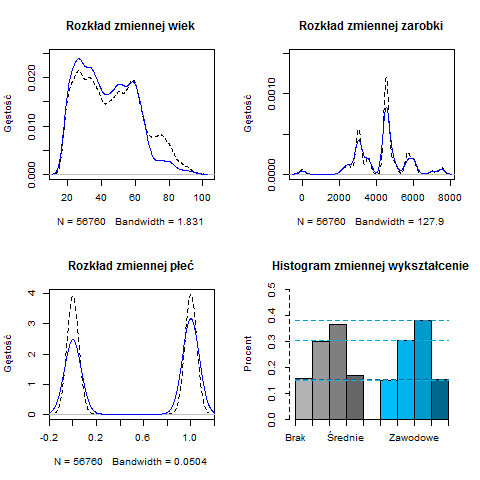
\includegraphics[width=\textwidth]{pictures/profile_klientow.png}
  \captionsetup{margin=10pt,font=small,labelfont=bf,width=.8\textwidth}
  \caption[Cechy konsumentów marki w porównaniu do wszystkich agentów]{Cechy konsumentów marki w porównaniu do wszystkich agentów (\textit{czarny} --- ogół klientów,\textit{niebieski} --- dla klientów marki). \textit{Źródło:} opracowanie własne.}\label{profile}
\end{figure}


\begin{figure}[hbt]
  \centering
    
\includegraphics[width=\textwidth]{../mapy/firma.png}
  \captionsetup{margin=10pt,font=small,labelfont=bf,width=.8\textwidth}
  \caption[Mapa z zaznaczonymi lokalizacjami jednostek przedsiębiorstwa]{Mapa z zaznaczonymi lokalizacjami jednostek przedsiębiorstwa (\textit{szary} --- drogi, \textit{pomarańczowy} --- sklepy, \textit{błękitny} -- fabryki, \textit{żółty} -- fabryki). \textit{Źródło:} opracowanie własne.}\label{mapafirma}
\end{figure}

\begin{figure}[hbt]
  \centering
    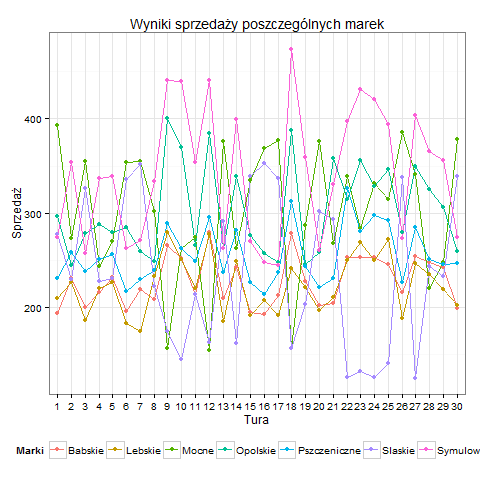
\includegraphics[width=\textwidth]{pictures/sprzedaz_marek.png}
  \captionsetup{margin=10pt,font=small,labelfont=bf,width=.8\textwidth}
  \caption[Statystyki sprzedaży marek symulowanych w modelu]{Statystyki sprzedaży marek symulowanych w modelu. \textit{Źródło:} opracowanie własne.}\label{fig:sprzedaz_marek}
\end{figure}


\begin{figure}[hbt]
  \centering

  \begin{subfigure}[t]{0.8\textwidth}
    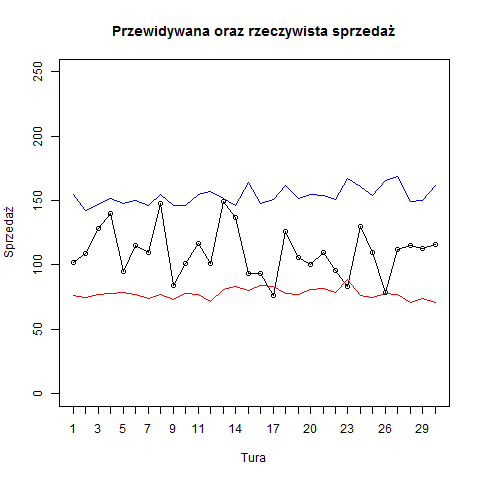
\includegraphics[width=\textwidth]{pictures/prognozy_lg_kn.png}
  \end{subfigure}
  \captionsetup{margin=10pt,font=small,labelfont=bf,width=.8\textwidth}

  \caption[Przewidywana i realna sprzedaż w modelu]{Przewidywana i realna sprzedaż w modelu (textit{niebieski} --- regresja logistyczna, \textit{czerwony} ---  $K$-neareast neighbours ). \textit{Źródło:} opracowanie własne.}\label{fig:prognozy_porowniania}
\end{figure}

\begin{figure}[hbt]
  \centering

  \begin{subfigure}[t]{0.8\textwidth}
    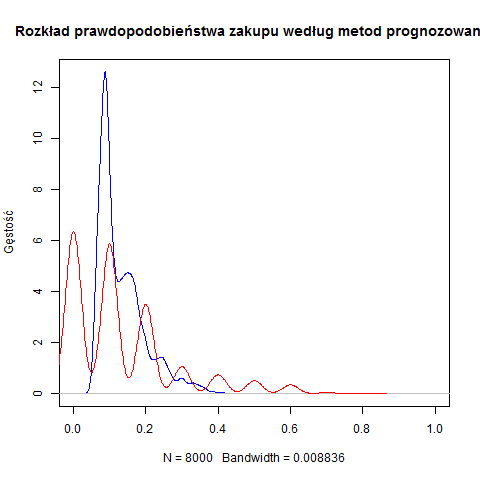
\includegraphics[width=\textwidth]{pictures/rozklad_prognoz}
  \end{subfigure}
  \captionsetup{margin=10pt,font=small,labelfont=bf,width=.8\textwidth}

  \caption[Rozkład prawdopodobieństwa zakupu w prognozach]{Rozkład prawdopodobieństwa zakupu w prognozach według metod prognoz. \textit{(regresja logistyczna --- niebieski, $K$-neareast neighbours --- czerwony)} \textit{Źródło:} opracowanie własne.}\label{fig:rozklad_lg_kn}
\end{figure}

\begin{figure}[hbt]
  \centering

  \begin{subfigure}[t]{0.8\textwidth}
    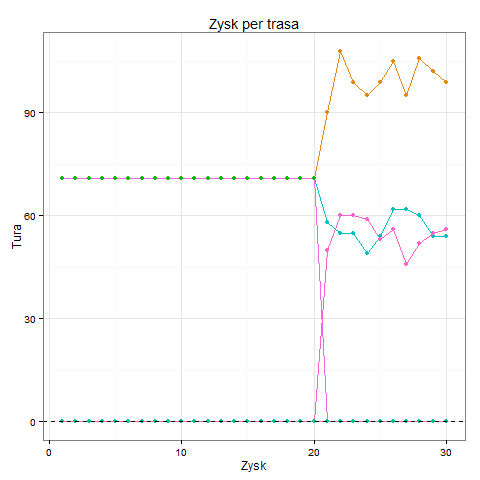
\includegraphics[width=\textwidth]{pictures/trasy.png}
  \end{subfigure}

  \captionsetup{margin=10pt,font=small,labelfont=bf,width=.8\textwidth}

  \caption[Alokacje wolumenów dostaw wśród możliwych ścieżek]{Alokacje wolumenów dostaw wśród możliwych ścieżek. Przerywana liniia oznacza inicjalizację działania modelu, kolory oznaczają różne trasy. \textit{Źródło:} opracowanie własne.}\label{fig:sciezki}
\end{figure}

\begin{figure}[hbt]
  \centering
  \begin{subfigure}[t]{0.6\textwidth}
    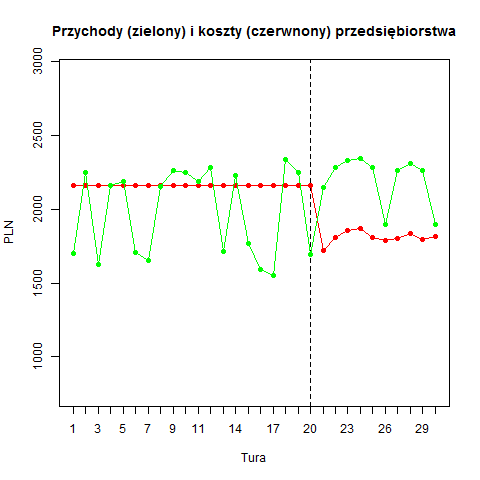
\includegraphics[width=\textwidth]{pictures/przychody_koszty_lm.png}
    \caption{Przychody i koszty symulowanego przedsiębiorstwa w symulacji z metodą prognozowania regresji logistycznej.}
    \label{fig:przychod_koszt}
  \end{subfigure}
  \hfill
  \begin{subfigure}[t]{0.6\textwidth}

    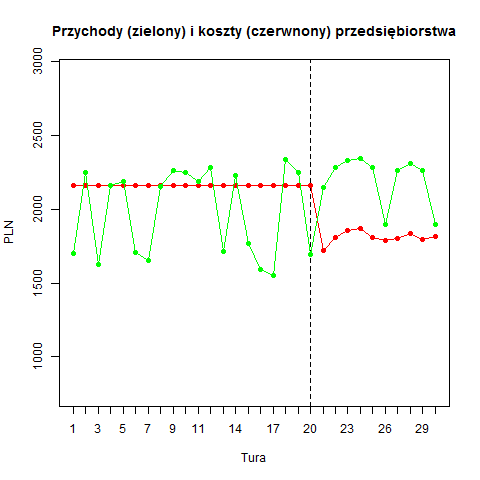
\includegraphics[width=\textwidth]{pictures/przcyhody_koszty_kn.png}
    \caption{Przychody i koszty symulowanego przedsiębiorstwa w symulacji z metodą prognozowania $K$-neareast neighbours.}
    \label{fig:zysk}
  \end{subfigure}
  
  \captionsetup{margin=10pt,font=small,labelfont=bf,width=.8\textwidth}

  \caption[Wyniki finansowe symulowanego przedsiębiorstwa w zależności od metody prognozowania]{Wyniki finansowe symulowanego przedsiębiorstwa w zależności od metody prognozowania. Przerywana linia oznacza inicjalizację algorytmu (\textit{zielony} --- przychody, \textit{czerwony} --- koszty). \textit{Źródło:} opracowanie własne.}\label{fig:wynikifin}
\end{figure}

\begin{figure}[hbt]
  \centering
  \begin{subfigure}[t]{0.6\textwidth}
    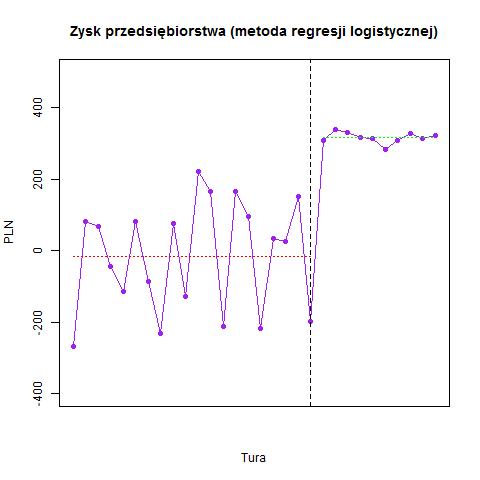
\includegraphics[width=\textwidth]{pictures/zysk_lm.png}
    \caption{Zysk symulowanego przedsiębiorstwa z metodą prognozowania regresji logistycznej.}
    \label{fig:przychod_koszt}
  \end{subfigure}
  \hfill
  \begin{subfigure}[t]{0.6\textwidth}

    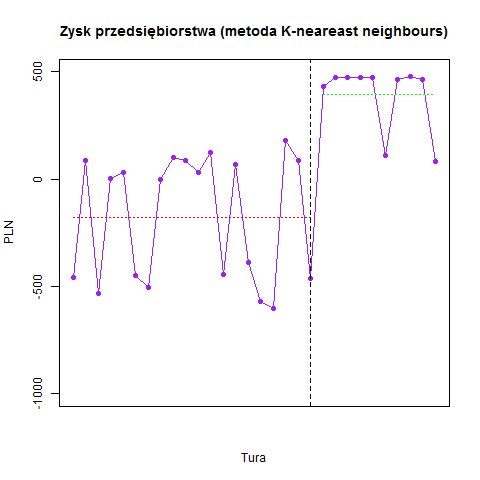
\includegraphics[width=\textwidth]{pictures/zysk_km.png}
    \caption{Zysk symulowanego przedsiębiorstwa w symulacji z metodą prognozowania $K$-neareast neighbours.}
    \label{fig:zysk}
  \end{subfigure}
  
  \captionsetup{margin=10pt,font=small,labelfont=bf,width=.8\textwidth}

  \caption[Zysk symulowanego przedsiębiorstwa w zależności od metody prognozowania]{Zysk symulowanego przedsiębiorstwa w zależności od metody prognozowania. Przerywana linia oznacza inicjalizację algorytmu (\textit{fioletowy} --- zysk, \textit{czerwony} --- średni zysk przed implementacji algorytmu, \textit{zielony} --- średni zysk po implementacji algorytmu). \textit{Źródło:} opracowanie własne.}\label{fig:wynikifin}
\end{figure}

% --- appendices ------------------------------------------------------
\appendix

% --- bibliography ----------------------------------------------------
\clearpage
\bibliographystyle{agsm}
\bibliography{refs}

% --- abstract --------------------------------------------------------
\clearpage
\addcontentsline{toc}{section}{Lista tablic}
\listoftables

% --- abstract --------------------------------------------------------
\clearpage
\addcontentsline{toc}{section}{Lista rysunków}
\listoffigures



% --- abstract --------------------------------------------------------
\clearpage
\addcontentsline{toc}{section}{Streszczenie}
\section*{Streszczenie}


Celem pracy jest zaproponowanie heurystyki optymalizacji podejmowania decyzji w przedsiębiorstwie na podstawie modelowania predyktywnego. Proponowany algorytm optymalizuje alokację wolumenów dostaw na wszystkie możliwe trasy dostaw, posługując się prognozami popytu uzyskanymi na podstawie przeszłej historii transakcji. 

W celu weryfikacji działania algorytmu zbudowany został model wieloagentowy, który symuluje lokalny rynek. Model w oparciu o lokalizację jednostek przedsiębiorstwa oraz konsumentów symuluje procesy logistyczny oraz decyzje konsumenckie. 

Wyniki działania algorytmu w opisywanym modelu sugerują, że jego zastosowanie w przedsiębiorstwach pozwala na zwiększenie rentowności przez dostosowanie wolumenu dostaw do popytu w każdym ze sklepów, oraz minimalizacji kosztów dostaw.

\end{document}

